\documentclass{article}
% ready for submission
%\usepackage{neurips_2023}


% to compile a preprint version, e.g., for submission to arXiv, add add the
% [preprint] option:
%     \usepackage[preprint]{neurips_2023}


% to compile a camera-ready version, add the [final] option, e.g.:
%     \usepackage[final]{neurips_2023}


% to avoid loading the natbib package, add option nonatbib:
    \usepackage[nonatbib,preprint]{neurips_2023}


\usepackage[utf8]{inputenc} % allow utf-8 input
\usepackage[T1]{fontenc}    % use 8-bit T1 fonts
\usepackage{hyperref}       % hyperlinks
\usepackage{url}            % simple URL typesetting
\usepackage{booktabs}       % professional-quality tables
\usepackage{amsfonts}       % blackboard math symbols
\usepackage{nicefrac}       % compact symbols for 1/2, etc.
\usepackage{microtype}      % microtypography
\usepackage{xcolor}         % colors
\usepackage[square,sort&compress]{natbib}
\bibliographystyle{abbrvnat}
%\usepackage{biblatex}
%\addbibresource{references.bib}
\usepackage{cleveref}
\usepackage{subcaption}
\usepackage{graphicx}
\usepackage{todonotes}
\usepackage{float}
\usepackage{multirow}

\newcommand{\beginsupplement}{%
        \setcounter{table}{0}
        \renewcommand{\thetable}{S\arabic{table}}%
        \setcounter{figure}{0}
        \renewcommand{\thefigure}{S\arabic{figure}}%
        \setcounter{section}{0}
        \renewcommand{\thesection}{\Roman{section}}%
        \setcounter{subsection}{0}
        \renewcommand{\thesubsection}{\Roman{section}.\arabic{subsection}}%

      }
     
\title{Receptive Field and Neural Networks Representations}


% The \author macro works with any number of authors. There are two commands
% used to separate the names and addresses of multiple authors: \And and \AND.
%
% Using \And between authors leaves it to LaTeX to determine where to break the
% lines. Using \AND forces a line break at that point. So, if LaTeX puts 3 of 4
% authors names on the first line, and the last on the second line, try using
% \AND instead of \And before the third author name.


\author{%
  Luis Alfredo Avendaño Muñoz.~\thanks{Use footnote for providing further information
    about author (webpage, alternative address)---\emph{not} for acknowledging
    funding agencies.} \\
  School of Computing\\
  University of Leeds\\
  Leeds, United Kingdom \\
  \texttt{sclaam@leeds.ac.uk} \\
  % examples of more authors
  % \And
  % Coauthor \\
  % Affiliation \\
  % Address \\
  % \texttt{email} \\
  % \AND
  % Coauthor \\
  % Affiliation \\
  % Address \\
  % \texttt{email} \\
  % \And
  % Coauthor \\
  % Affiliation \\
  % Address \\
  % \texttt{email} \\
  % \And
  % Coauthor \\
  % Affiliation \\
  % Address \\
  % \texttt{email} \\
}



\begin{document}


\maketitle


\begin{abstract}
\end{abstract}

\section{Introduction}
%\begin{itemize}
%
% \item Neural networks learn hierarchical features (some citations), They are able learn different levels of features
%   and integrate them correctly for the task at hand (deep learning book citation or Yan Lecunn lectures object
%   detectors in scene classifiers)
%   \item The receptive field of a model is known to be related to how the representations of neural networks are formed
%     yet, their relationship is still not well understood.
%   \item Additionally, the effect of the receptive field on the loss landscape of neural networks has not been
%     investigated (to the best of our knowledge)
%
%     \item In this paper we explore the relationship between the receptive field of neural networks and their loss
%       landscape. We show that larger receptive fields are not necessarily better for performance in image
%       classification. But instead, we show that they are important for learning features robust to pruning.
%\end{itemize}
%

Neural networks have emerged as the standard approach for a wide range of applications, ranging from image recognition
\citep{dengImageNetLargescaleHierarchical2009} to natural language processing \citep{devlinBERTPretrainingDeep2019} and speech synthesis
\citep{oordWaveNetGenerativeModel2016,lecunDeepLearning2015}.
% Pruning Part of the introduction
%However, as neural networks become
%increasingly complex, they demand more computing power and memory resources \citep{brownLanguageModelsAre2020,
%thompsonComputationalLimitsDeep2020} This has led to an escalating interest in compression techniques that can retain or efficiently recover performance while reducing the size of neural networks.
%%%%%%%
Neural networks owe their expressiveness to the ability to learn hierarchical features and representations form the data
that are particularly suited for the task at hand \citep{goodfellowDeepLearning2016}. These features are influenced by
the highly non-linear.



The reason that make neural networks so good is the features that they learn from the data
(\citep{zhouObjectDetectorsEmerge2015}),
They learning general features in the first layers while in deeper layer they integrate and combine the simpler features and create
more complex and detailed features. One aspect that greatly affects these representations, as well as training dynamics is the receptive field of
neural networks, yet, its effect on the representations remains not fully understood.


In this paper we systematically explore the relationship that the receptive field has with the representations of neural networks
along with the loss landscape these models. We show that if we manipulate the receptive field by changing the kernel
size of the first maxpooling layer leaving every other component static we can demonstrate that the models losses
generalization capacity as we increase the receptive field. Surprisingly, for high levels of pruning, it turns out
that the negative effect on accuracy have an inverse relationship with the receptive field. We show that the
receptive fields greatly affects the loss landscape of the models as shown by the Hessian spectra at initialisation.

We empirically validated our results with two different type of models  with similar number of parameters (VGG-like and
Resnet50) and two different datasets with different image sizes,( CIFAR10 and Tiny imagenet)

Our contributions are:
\begin{itemize}
  %\item We show that the receptive field greatly affects the loss landscape defining the type of features that of these models an be
  %  learning and in consequence affecting the robustness of the networks against pruning
  \item We show that the receptive field is linked to the "ruggedness" of the loss landscape of neural networks
    affecting its trainability and the robustness of its representations to pruning.
  \item
\end{itemize}



\section{Related Work}
\textbf{Receptive field literature}
\begin{itemize}
  \item \cite{luoUnderstandingEffectiveReceptive2016}
    \item object detectors \cite{zhouObjectDetectorsEmerge2015}
      \item Interpretation of ResNet by Visualization of Preferred Stimulus in Receptive Fields \cite{kobayashiInterpretationResNetVisualization2020}
\end{itemize}
\textbf{Landscape investigation}
\begin{itemize}
  \item On the Relation Between the Sharpest Directions of DNN Loss and the SGD Step Length \cite{jastrzebskiRelationSharpestDirections2019}
\end{itemize}

\section{Experimental results}


 In this section we empirically investigate the effect that the receptive field has in a network's trainability and
 prunability. We Statistically validate our results on VGG and ReseNet50 architecture and in CIFAR10 and Tiny ImageNet
 datasets. 


 \todo[inline]{Here I never talked of how I calculated the receptive field, which I used a libary that calculates
 the gradient projection in a dummy input space with a projected gradient of 1 in the middle of all the fueature maps of the
last convolutional layer for the two architectures.
}


\subsection{Experimental settings}
We used a custom implementation of the ResNet50 and VGG models with a modified maxpooling layer after the first
convolutional layer for manipulating the receptive field. Implementation details are in \Cref{sebsec:implementation_details}. The dataset are CIFAR10 and Tiny ImageNet. The training hyperparameters are the following:
\begin{itemize}
  \setlength\itemsep{.0em}
    \item Epochs: 200
    \item Optimizer: SGD
    \item Learning rate: 0.0001
    \item Learning rate schedule: Cosine annealing with $T_{max}=200$ 
    \item Momentum: 0.9
    \item Weight Decay: $5 \times 10^{-5}$
    \item Gradient clipping: 0.1
\end{itemize}


\subsection{Manipulating the Receptive Field}

There is plentiful of ways for Manipulating the receptive field. It is known that the presence of skip connections
affect the receptive fields along with depth and dilation on convolutions. We wanted to alter the receptive field
minimum alterations to the rest of the networks leaving all layers with the exact same number of parameters. We placed a
maxpooling layer just after the first convolutional layer on both architectures and we changed the kernel size of that
layer. That is the only difference between the different models on each experiment. For each
architecture-dataset-receptive field combination we trained 5 models and the result are shown in \ref{sec:rfanda}.
\subsection{Receptive Field, Accuracy and Pruning}
\label{sec:rfanda}
Here we show the dense accuracy after training the models and its one-shot pruned accuracy. One interesting observation
is that larger receptive field correlates with lower accuracy but simultaneously its one-shot pruning performances is
better than those for smaller receptive fields. This behaviour generalises across all the combinations of
architecture-dataset. In \Cref{subsec:OneShotPruningRates} we show that the current trend in accuracy (for dense and prune version) only
arises for sufficiently large pruning rate (>0.8). We also fine-tuned the models to test their real-world application
capabilities as seen  in \Cref{subsec:Fine_tuning_solutions} but here we only show the pruning rate of 0.9 as means to
show the one-shot behaviour of these networks in order to understand their one-shot potential.
For each one of the combinations shown here we trained and pruned 5 models, the values presented are the mean  with its
standard deviation.

The image size for CIFAR10 and Tiny ImageNet is 32x32 and  64x64 respectively. In both cases the receptive fields of
each architecture is greater than the size of the image.

% Please add the following required packages to your document preamble:
% \usepackage{booktabs}
\begin{table}[H]
  \centering
\begin{tabular}{@{}cccc@{}}
\toprule
\multicolumn{4}{c}{\textbf{VGG Accuracy}}                                                                                                                                                                          \\ \midrule
\multicolumn{1}{l}{\textbf{Receptive Field}} & \multicolumn{1}{l}{\textbf{Dense}} & \multicolumn{1}{l}{\textbf{Pruned
(90\%)}} & \multicolumn{1}{l}{\textbf{Difference in Accuracy}} \\
181                                          & 93.5 $\pm$ 0.11                                  & 10.9 $\pm$2.03                                    & 82.6 $\pm$ 2.02                                     \\
359                                          & 91.1 $\pm$ 0.23                                  & 32.4 $\pm$ 15.7                                   & 58.7 $\pm$ 15.8                                     \\
537                                          & 87.8 $\pm$ 0.19                                  & 87.6 $\pm$ 0.30                                   & 0.18 $\pm$ 0.16                                     \\
715                                          & 85.8 $\pm$ 0.21                                  & 85.8 $\pm$ 0.22                                   & 0.07 $\pm$ 0.04                                     \\ \midrule
\multicolumn{4}{c}{\textbf{ResNet 50 Accuracy}}                                                                                                                                                                    \\ \midrule
\multicolumn{1}{l}{\textbf{Receptive Field}} & \multicolumn{1}{l}{\textbf{Dense}} & \multicolumn{1}{l}{\textbf{Pruned
(90\%)}} & \multicolumn{1}{l}{\textbf{Difference in Accuracy}} \\
110                                          & 94.8 $\pm$ 0.29                                  & 56 $\pm$ 20.7                                     & 38.7 $\pm$ 20.5                                     \\
213                                          & 94.0 $\pm$ 0.16                                  & 91.7 $\pm$ 0.98                                   & 2.25 $\pm$ 0.90                                     \\
318                                          & 92.2 $\pm$ 0.18                                  & 91.4 $\pm$ 0.45                                   & 0.85 $\pm$ 0.49                                     \\
423                                          & 90.4 $\pm$  0.30                                 & 90.2 $\pm$ 0.37
                                             & 0.18 $\pm$ 0.09                                     \\ \bottomrule
                                             \\
\end{tabular}
\caption{\textbf{CIFAR10 results:} Here are summarised the results for the experiments performed in CIFAR10. It can be
  seen that the discrepancy in accuracy between different receptive fields is consistent for these two architectures.
  Also, as we increase the receptive field we can see that the gap in performance between dense and pruned models
diminishes. The pruning rate used is 90\%}
\label{tab:pruned_cifar10}
\end{table}


\begin{table}[H]
  \centering
\begin{tabular}{crrr}\toprule
  \multicolumn{4}{c}{\textbf{VGG Accuracy}}                                                                                                                                                                          \\ \hline \multicolumn{1}{l}{\textbf{Receptive Field}}& \multicolumn{1}{l}{\textbf{Dense}}  & \multicolumn{1}{l}{\textbf{Pruned}}  & \multicolumn{1}{l}{\textbf{Difference in Accuracy}} \\
181& 61.5 $\pm$ 0.33& 0.75 $\pm$0.09 & 60.8 $\pm$ 0.32\\
359& 53.2 $\pm$ 0.20& 0.63 $\pm$ 0.17& 52.6 $\pm$ 0.36\\
537& 41.0 $\pm$ 1.91& 16.7 $\pm$ 7.50& 24.3 $\pm$ 5.81\\
715& 38.5 $\pm$ 1.69& 21.8 $\pm$ 6.57& 16.7 $\pm$ 7.21\\ \hline
\multicolumn{4}{c}{\textbf{ResNet 50 Accuracy}}                                                                                                                                                                    \\ \hline
\multicolumn{1}{l}{\textbf{Receptive Field}}& \multicolumn{1}{l}{\textbf{Dense}} & \multicolumn{1}{l}{\textbf{Pruned}}  & \multicolumn{1}{l}{\textbf{Difference in Accuracy}} \\
213                                         & 61.8 $\pm$ 0.40                                  & 5.91 $\pm$ 0.89                                    & 55.9 $\pm$ 0.99                                     \\
318                                         & 59.1 $\pm$ 0.36                                  & 8.56 $\pm$ 2.66                                    & 50.5 $\pm$ 2.55                                     \\
423                                         & 56.5 $\pm$ 0.27                                  & 21.4 $\pm$ 2.87                                     & 35.0 $\pm$ 2.99                                     \\ \hline\\
\end{tabular}\\
\caption{ \textbf{Tiny ImageNet Results:} Here are summarised the results for the experiments performed in Tiny ImageNet.
Similarly to CIFAR10, the trend of diminishing dense accuracy and gap between dense and pruned accuracy as we increase
the receptive field is consistent in the two architectures.
The pruning rate is 90\%  excluding the first convolutional layer and the linear layer}
\label{tab:tiny_imagenet_results}
\end{table}

\subsection{Fine-tuning Pruned Solutions}
\label{subsec:Fine_tuning_solutions}
Here we fine-tuned the pruned solutions while preserving the mask for 10 epochs with the following hyper-parameters
\begin{itemize}
  \item Initial Learning Rate: 0.0001,
  \item Weight Decay:5e-4
  \item Momentum:0,9
  \item Gradient clip: 0.1
\end{itemize}

%\todo[inline]{All of the following figures would be better on a table}
% Please add the following required packages to your document preamble:
% \usepackage{booktabs}
\begin{table}[H]
  \centering
\begin{tabular}{@{}cccc@{}}
\toprule
\multicolumn{4}{c}{\textbf{VGG  Accuracy}}                                                                                                                                  \\ \midrule
\textbf{Receptive Field} & \textbf{Dense} & \multicolumn{1}{l}{\textbf{Pruned (90\%)}} & \multicolumn{1}{l}{\textbf{Difference In Accuracy}} \\ \midrule
181                      & 93.52$\pm$0.115              & 91.42$\pm$2.026                                   & 2.106$\pm$2.111                                     \\
359                      & 91.15$\pm$0.232              & 90.81$\pm$0.293                                   & 0.348$\pm$0.366                                     \\
537                      & 87.88$\pm$0.193              & 87.85$\pm$0.223                                   & 0.032$\pm$0.070                                     \\
715                      & 85.88$\pm$0.217              & 85.78$\pm$0.286                                   & 0.096$\pm$0.140                                     \\ \midrule
\multicolumn{4}{c}{\textbf{ResNet50 Accuracy}}                                                                                                                             \\ \midrule
\textbf{Receptive Field} & \textbf{Dense Test Accuracy} & \textbf{Pruned (90\%)}                     & \textbf{Difference In Accuracy}                     \\
110                      & 94.69$\pm$0.213              & 90.86$\pm$0.701                                   & 3.830$\pm$0.795                                     \\
213                      & 94.03$\pm$0.236              & 93.55$\pm$0.211                                   & 0.477$\pm$0.197                                     \\
318                      & 92.22$\pm$0.244              & 92.03$\pm$0.200                                   & 0.190$\pm$0.053                                     \\
423                      & 90.23$\pm$0.169              & 90.23$\pm$0.147                                   &
-0.007$\pm$0.087                                    \\ \bottomrule\\
\end{tabular}
\caption{VGG and ResNet50 on CIFAR10 with fine tuning and pruning rate 0.9}
\label{tab:cifar10 fine tuning pruning rate 09}
\end{table}


% Please add the following required packages to your document preamble:
% \usepackage{booktabs}
\begin{table}[H]
  \centering
\begin{tabular}{@{}cccc@{}}
\toprule
\multicolumn{4}{c}{\textbf{VGG}}                                                                                                                                  \\ \midrule
\textbf{Receptive Field} & \textbf{Dense Test Accuracy} & \multicolumn{1}{l}{\textbf{Pruned (90\%)}} & \multicolumn{1}{l}{\textbf{Difference In Accuracy}} \\ \midrule
181                      & 61.58$\pm$0.333              & 30.21$\pm$2.595                                   & 31.37$\pm$2.534                                     \\
359                      & 53.25$\pm$0.207              & 3.558$\pm$2.027                                   & 49.69$\pm$2.188                                     \\
537                      & 41.05$\pm$1.917              & 38.21$\pm$2.699                                   & 2.842$\pm$0.884                                     \\
715                      & 38.57$\pm$1.691              & 36.45$\pm$1.549                                   & 2.126$\pm$0.762                                     \\ \midrule
\multicolumn{4}{c}{\textbf{ResNet50}}                                                                                                                             \\ \midrule
\textbf{Receptive Field} & \textbf{Dense Test Accuracy} & \textbf{Pruned (90\%)}                     & \textbf{Difference In Accuracy}                     \\
213                      & 61.83$\pm$0.401              & 44.56$\pm$1.205                                   & 17.27$\pm$1.346                                     \\
318                      & 59.10$\pm$0.368              & 44.28$\pm$0.648                                   & 14.82$\pm$0.633                                     \\
423                      & 56.53$\pm$0.279              & 46.16$\pm$0.716                                   &
10.37$\pm$0.577                                     \\ \bottomrule \\
\end{tabular}
\caption{VGG and ReseNet50 on Tiny ImageNet with fine tuning and pruning rate of 0.9}
\label{tab:cifar10 fine tuning pruning rate 09}
\end{table}

\textbf{ Tiny ImageNet for 100 Epochs}
% Please add the following required packages to your document preamble:
% \usepackage{booktabs}
\begin{table}[H]
  \centering
\begin{tabular}{@{}cccc@{}}
\toprule
\multicolumn{4}{c}{\textbf{VGG  Test Accuracy}}                                                                    \\ \midrule
\textbf{Receptive Field} & \textbf{Dense}  & \textbf{Pruned (90\%)} & \multicolumn{1}{l}{\textbf{Difference In Accuracy}} \\ \midrule
181                      & 61.58$\pm$0.333 & 33.93$\pm$0.320 & 27.66$\pm$0.521                                     \\
359                      & 53.25$\pm$0.207 & 29.73$\pm$16.15 & 23.52$\pm$16.23                                     \\
537                      & 41.05$\pm$1.917 & 37.50$\pm$1.916 & 3.554$\pm$0.164                                     \\
715                      & 38.57$\pm$1.691 & 35.50$\pm$1.812 & 3.078$\pm$0.453                                     \\ \midrule
\multicolumn{4}{c}{\textbf{ResNet50 Test Accuracy}}                                                                \\ \midrule
\textbf{Receptive Field} & \textbf{Dense}  & \textbf{Pruned (90\%)} & \textbf{Difference In Accuracy}                     \\
\midrule
213                      & 61.83$\pm$0.401 & 50.21$\pm$0.428 & 11.62$\pm$0.487                                     \\
318                      & 59.10$\pm$0.368 & 49.83$\pm$0.583 & 9.274$\pm$0.413                                     \\
423                      & 56.53$\pm$0.279 & 49.43$\pm$0.403 & 7.106$\pm$0.361                                     \\
\bottomrule \\
\end{tabular}
\caption{VGG and ReseNet50 on Tiny ImageNet with fine tuning for 100 epochs and pruning rate of 0.9}
\label{tab:tiny imagenet fine tuning pruning rate 09}
\end{table}




\subsection{Loss Landscape and Receptive Field}

Why do models with large receptive field behave in this manner? One hypothesis is that the loss landscape changes in
such a way that makes more difficult for SGD to found a better solution. In \Cref{fig:hessian_vgg_cifar10,fig:hessian_resnet50_cifar10} we show the 90 largest eigen values for both models on CIFAR10, before and after training. As
we can see, at the beginning of training the Hessian spectra of models with alter receptive field are wider and
encompass larger eigen values. This means that the landscape of that models has much more steeper directions of descent
(and ascent) making the landscape more chaotic  and difficult to traverse than for smaller receptive fields (maybe search
a citation that corroborates this?).

\todo[inline]{Talk about the training trajectory in \Cref{fig:training_trajectories}, and mention that the figures in
\Cref{fig:hessian_vgg_cifar10,fig:hessian_resnet50_cifar10} explain such behaviour. In \Cref{fig:images-resnet50_CIFAR10_training-png}
I trained for double the epochs trying to show that even with more training the
larger receptive field cannot match the smaller receptive field. The bump seen arround 200 epochs is due tu the learning
rate schedule, which is a cosine schedule with Tmax=200, right now im training a model with Tmax=400 to see if it that
claim is still valid. All the accuracies seen throughtout the document correspond to the best model while trainig
e.g. the bump}



\begin{figure}[!htp]
 \centering
     \begin{subfigure}[b]{0.45\textwidth}
    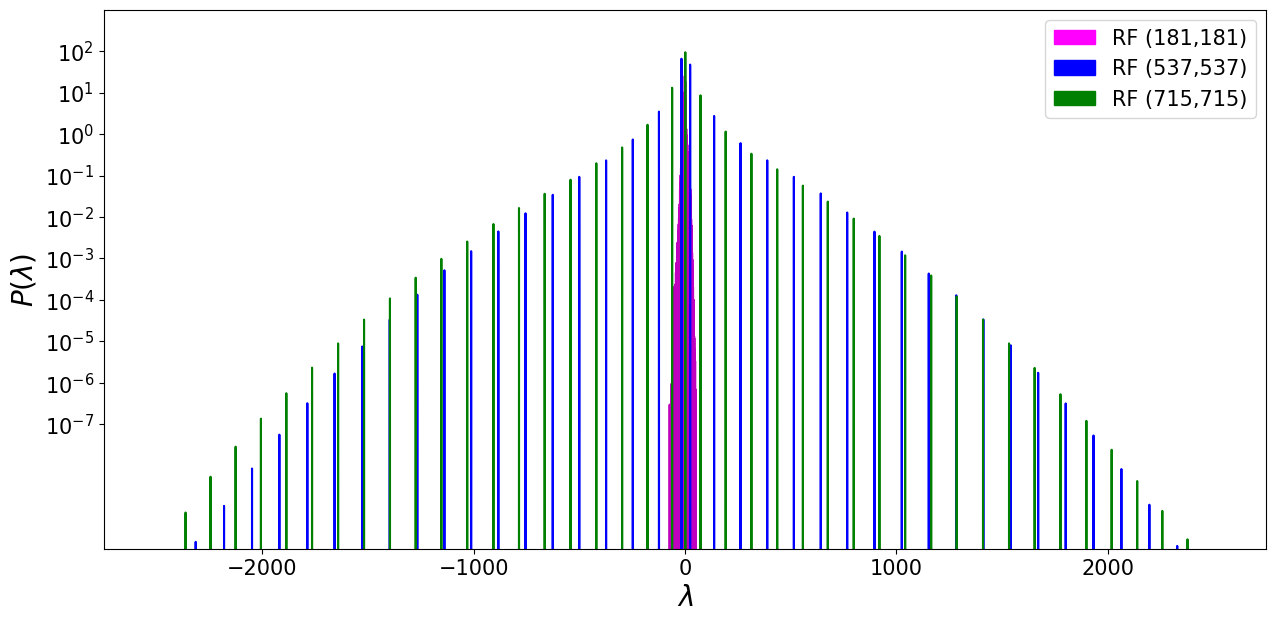
\includegraphics[width=7cm]{images/Hessian_spectre_vgg19_init_cifar10.png}
    \caption{Before Training}
    \label{subfig:Hessian_VGG_before_training}
     \end{subfigure}
      \hfill
     \begin{subfigure}[b]{0.45\textwidth}
    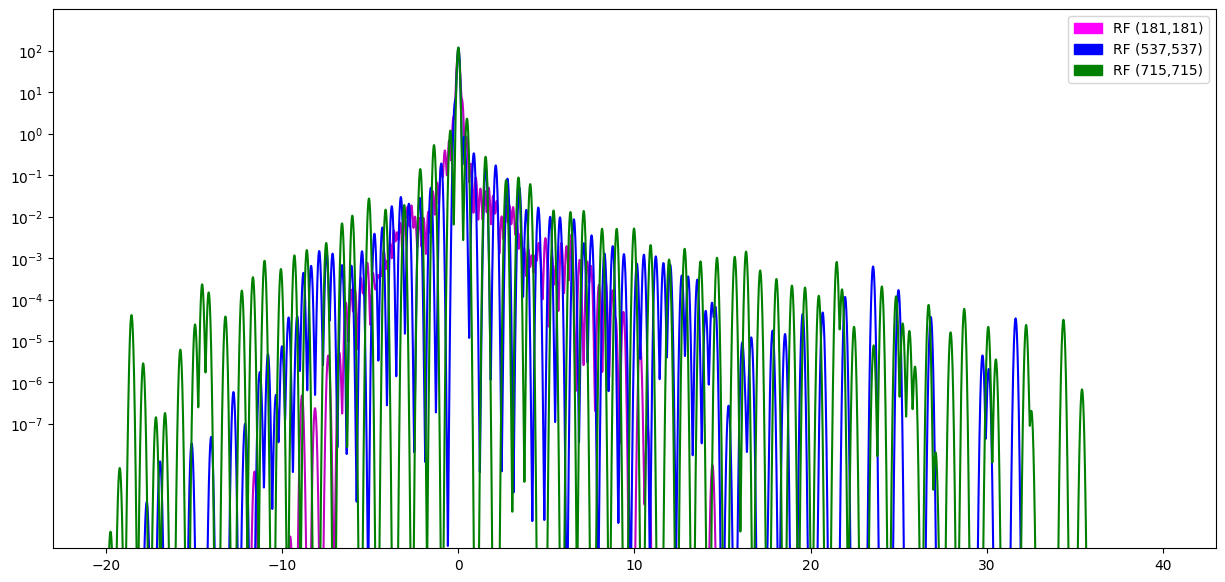
\includegraphics[width=7cm]{images/Hessian_spectre_vgg19_trained_cifar10.png}
    \caption{After training}
    \label{subfig:Hessian_VGG_after_training}
     \end{subfigure}
     \caption{Largest 90 eigen values of VGG model on CIFAR10 for different Receptive Fields \todo[inline]{Here I can
         put labels
     like $\lambda$ and $P(\lambda)$. Larger font} }
    \label{fig:hessian_vgg_cifar10}
\end{figure}
\begin{figure}[!htp]
 \centering
     \begin{subfigure}[b]{0.45\textwidth}
    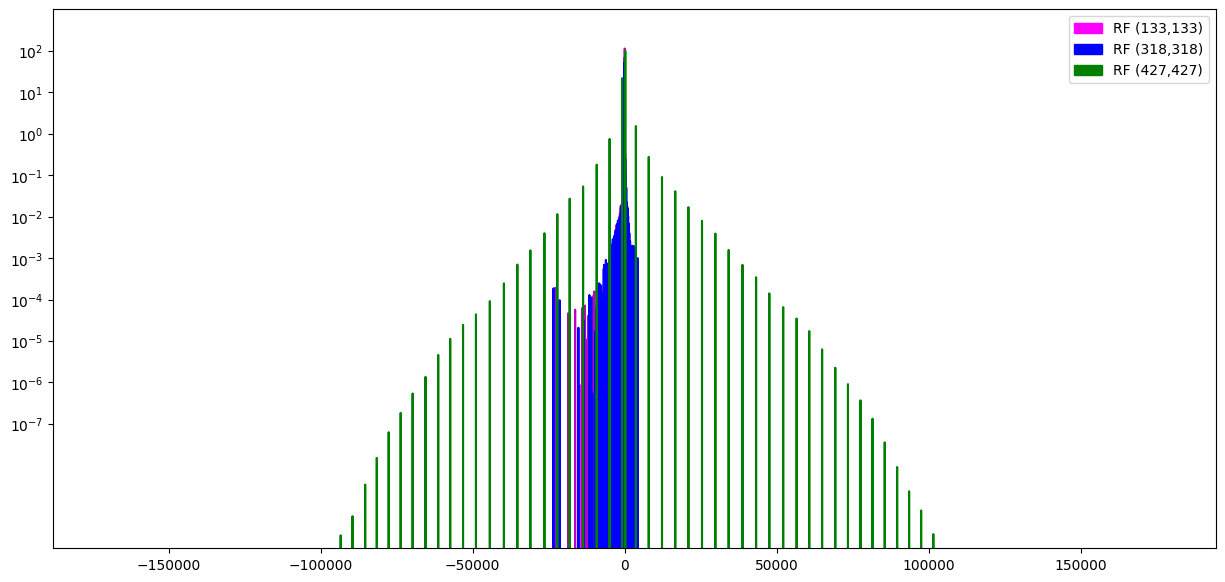
\includegraphics[width=7cm]{images/Hessian_spectre_resnet50_init_cifar10.png}
    \caption{Before Training}
    \label{subfig:}
     \end{subfigure}
      \hfill
     \begin{subfigure}[b]{0.45\textwidth}
    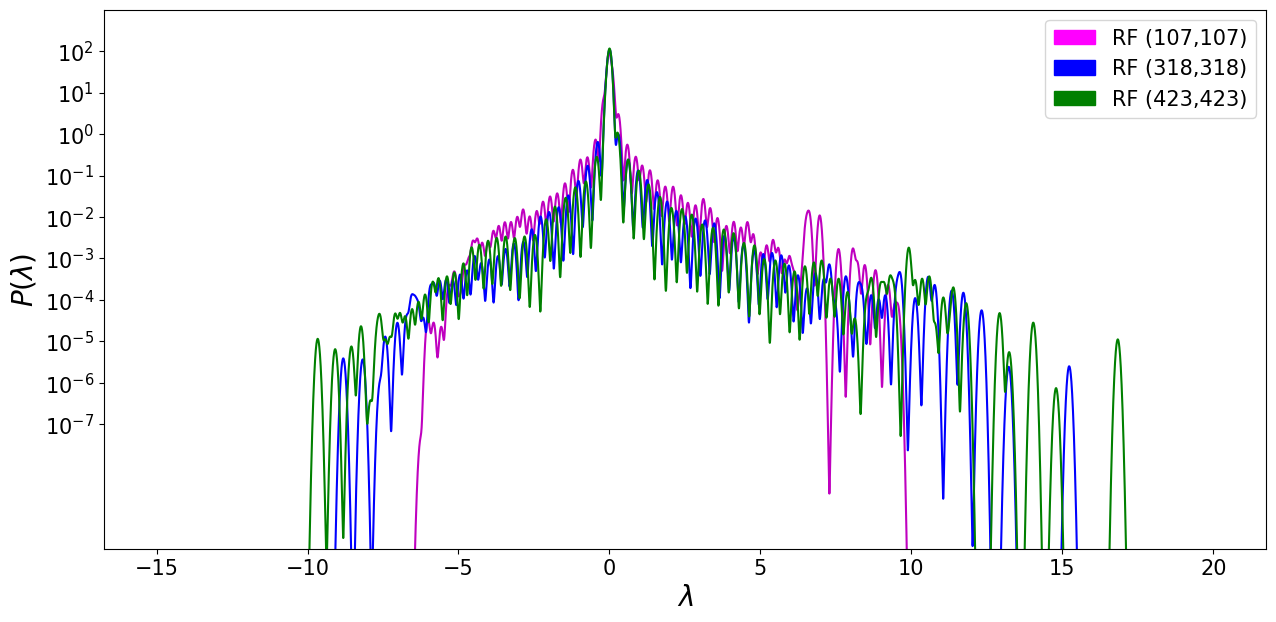
\includegraphics[width=7cm]{images/Hessian_spectre_resnet50_trained_cifar10.png}
    \caption{After training}
    \label{subfig:}
     \end{subfigure}
     \caption{Largest 90 eigen values of ResNet50 model on CIFAR10 for different Receptive Fields }
    \label{fig:hessian_resnet50_cifar10}
\end{figure}
\begin{figure}[!htp]
  \begin{subfigure}[b]{0.45\textwidth}
      \centering
      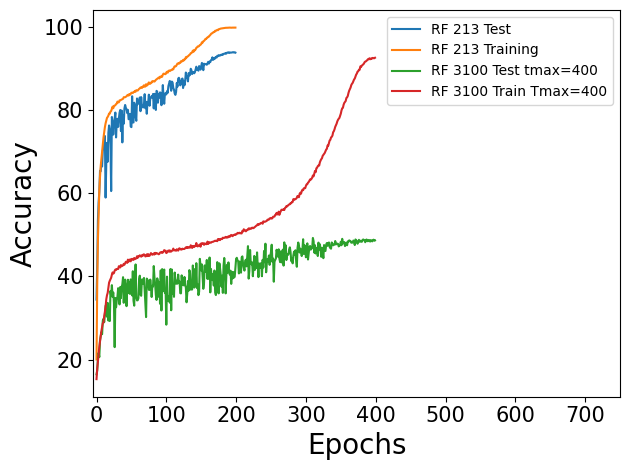
\includegraphics[width=7cm]{images/resnet50_CIFAR10_training.png}
      \caption{ResNet50 training for different Receptive fields on CIFAR10}
      \label{fig:images-resnet50_CIFAR10_training-png}
    \end{subfigure}
    \hfill
    \begin{subfigure}[b]{0.45\textwidth}
      \centering
      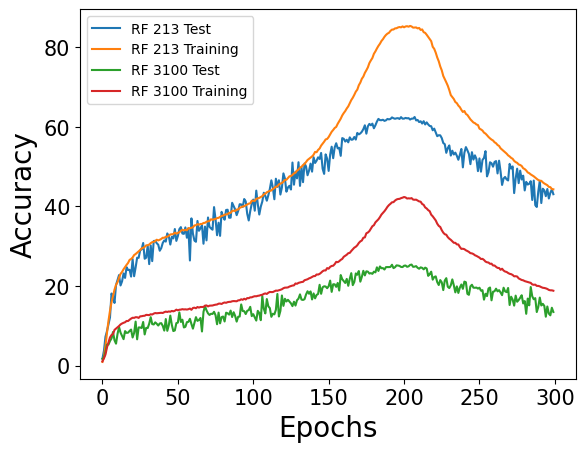
\includegraphics[width=7cm]{images/resnet50_Tiny_imagenet_training.png}
      \caption{ResNet50 training for different Receptive fields on Tiny ImageNet}
      \label{fig:images-resnet50_Tiny_imagenet_training-png}
    \end{subfigure}
     \caption{Training of ResNet50 on CIFAR10 and Tiny ImageNet}
     \label{fig:training_trajectories}
\end{figure}
But how does this affect the features or representations that these models learn? Next we show the similarity of the
internal representation two different seeds of the ReseNet50 model on CIFAR10., It is observed that the introduction of
larger receptive fields results in a divergence of representations within the deepest layers. This phenomenon can be
attributed to the heightened "chaotic" nature of the loss landscape, as indicated by the Hessian spectra in \Cref{fig:hessian_resnet50_cifar10}, particularly in instances where larger receptive fields are employed. Notably, the
representations in deeper layers for individual seeds exhibit dissimilarity, as they tend to converge into distinct
basins, differing not only from the majority of the network but also from corresponding layers in other seeds. The representation
 similarly was calculated using the first 1000 images of the test set and we use the Centred linear Kernel Alignment
 \citep{kornblithSimilarityNeuralNetwork2019} as similarity measure.
\begin{figure}[!htp]
        \centering
        \begin{subfigure}[b]{0.475\textwidth}
            \centering
            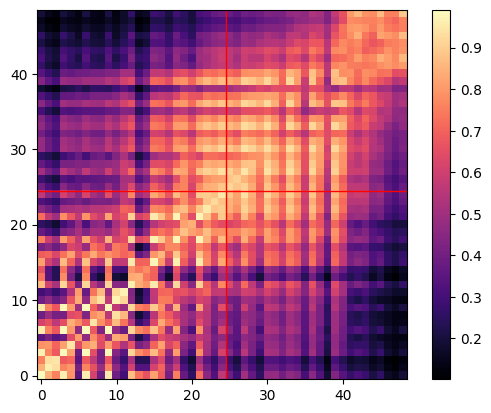
\includegraphics[width=0.7\textwidth]{images/resnet50_level1_similarity_cifar10.png}
            \caption[Network1]%
            {{\small Receptive Field 110}}    
            \label{fig:similarity_lvl1}
        \end{subfigure}
        \hfill
        \begin{subfigure}[b]{0.475\textwidth}  
            \centering 
            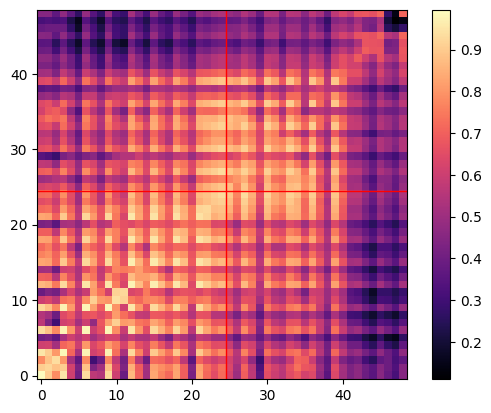
\includegraphics[width=0.7\textwidth]{images/resnet50_level2_similarity_cifar10.png}
            \caption[Network2]%
            {{\small Receptive Field 213}}    
            \label{fig:similarity_lvl2}
        \end{subfigure}
        \vskip\baselineskip
        \begin{subfigure}[b]{0.475\textwidth}   
            \centering 
            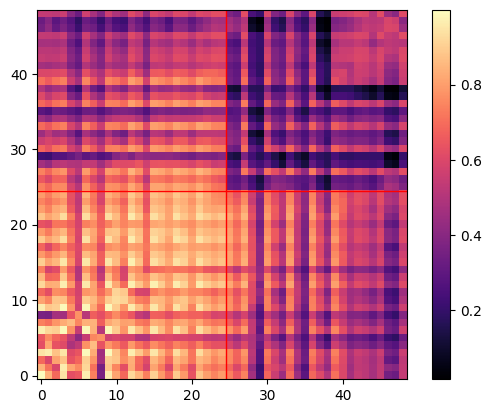
\includegraphics[width=0.7\textwidth]{images/resnet50_level3_similarity_cifar10.png}
            \caption[]%
            {{\small Receptive Field 318}}    
            \label{fig:similarity_lvl3}
        \end{subfigure}
        \hfill
        \begin{subfigure}[b]{0.475\textwidth}   
            \centering 
            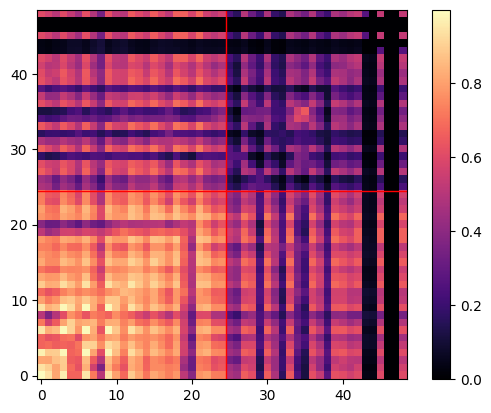
\includegraphics[width=0.7\textwidth]{images/resnet50_level4_similarity_cifar10.png}
            \caption[]%
            {{\small Receptive Field 423}}    
            \label{fig:similarity_lvl4}
        \end{subfigure}
        \caption[Representation similarity]
        {\small Representation similarly for all convolutional layers in ReseNet50 for different receptive fields. The red lines
        represent the middle layer of the model (25$^{\textrm{th}}$ layer). The largest receptive field (bottom right)
      has high degree of dissimilarity between its deeper layer representations when compared with the smallest
    receptive field (top left)}
        \label{fig:similarity_resenet50}
    \end{figure}

In \Cref{fig:similarity_resenet50} we can see that the similarity between layers decreases as we increase the receptive
field. This is consistent with our findings that the loss landscape for large receptive fields are more ``rugged''
(see \Cref{fig:hessian_resnet50_cifar10,fig:hessian_vgg_cifar10})
meaning that deeper layers, which learn specific features for the task \citep{yosinskiHowTransferableAre2014, roAutoLRLayerwisePruning2021}, converge to a more varied set of representations thus the
increase in dissimilarity. The shallow layers in the other hand, the representations between solutions converge to a
more uniform set of representations, hence their similarity. This is congruent with the notion that shallow layer
learn ``general'' features that are beneficial for transfer learning \citep{roAutoLRLayerwisePruning2021}.
Conversely, smaller receptive fields have a smoother loss landscape and in consequence, even the deeper, specific layers
in the network converge to similar representations. Another explanation is that due to the size of the receptive
field, the network's ability to learn nuanced features (those that normally would be learned in deeper layers) is
impaired, thus affecting its performance and similarities.

\subsection{Large Receptive Field for Tiny ImageNet}
\label{subsec:LargeRFTI}
% Please add the following required packages to your document preamble:
% \usepackage{booktabs}
\begin{table}[H]
  \centering
\begin{tabular}{@{}cccc@{}}\toprule
\multicolumn{4}{c}{\textbf{ResNet50 Test Accuracy}}                                            \\ \midrule
\textbf{Receptive Field} & \textbf{Dense}  & \textbf{Pruned (90\% One Shot)} & \textbf{Difference In Accuracy} \\ \midrule
1415                     & 32.00$\pm$0.192 & 32.00$\pm$0.192 & 0.000$\pm$0.000                 \\
1920                     & 29.28$\pm$0.627 & 29.28$\pm$0.627 & 0.000$\pm$0.000                 \\
3100                     & 22.84$\pm$0.370 & 22.84$\pm$0.370 & 0.000$\pm$0.000                 \\ \bottomrule
\end{tabular}
\caption{ReseNet50 with large Receptive Field on Tiny ImageNet  with pruning rate of 0.9}
\label{tab:tiny imagenet largeRF one shot pruning rate 09}
\end{table}

\subsection{Large Receptive Field for CIFAR10}
\label{subsec:LargeRFCF10}
% Please add the following required packages to your document preamble:
% \usepackage{booktabs}

\begin{table}[H]
  \centering
\begin{tabular}{@{}cccc@{}}
\toprule
\multicolumn{4}{c}{\textbf{ResNet50 Accuracy}}                                                                                         \\ \midrule
\textbf{Receptive Field} & \textbf{Dense}  & \multicolumn{1}{l}{\textbf{Pruned (90\% One Shot)}} & \multicolumn{1}{l}{\textbf{Difference in Accuracy}} \\ \midrule
1415                     & 72.87$\pm$0.787 & 72.87$\pm$0.787                     & 0.000$\pm$0.000                                     \\
1920                     & 53.37$\pm$1.293 & 53.37$\pm$1.293                     & 0.000$\pm$0.000                                     \\
3100                     & 50.11$\pm$0.256 & 50.11$\pm$0.256                     & 0.000$\pm$0.000
\\ \bottomrule \\
\end{tabular}
\caption{ReseNet50 with large receptive field in CIFAR10}
\label{tab:cifar10  largeRF one shot pruning rate 09}
\end{table}



\subsection{Width and Depth cannot Recover Information}

One question is : Is the information from the receptive field not recoverable by the width or depth of the model? To
answer this, we modified the width of ResNet50 by 2x and 3x times and found that despite the marginal improvement in performance, the width
of the model cannot retrieve all the information lost by the large receptive field, thus diverging from the observation that
accurate information can be extracted by coarsely tuned units \citep{ballardParallelVisualComputation1983}.


% Please add the following required packages to your document preamble:
% \usepackage{booktabs}
% \usepackage{multirow}
\begin{table}[H]
  \centering
\begin{tabular}{@{}cccc@{}}
\toprule
\textbf{Receptive Field} & \textbf{Width} & \textbf{Test Accuracy} & \multicolumn{1}{l}{\textbf{Original Test
Accuracy (Width=$\times1$)}} \\ \midrule
\multirow{2}{0}{3100}    & $\times2$             & 26.33                        & \multirow{2}{0}{22.84$\pm$0.370}                    \\
                         & $\times3$             & 26.04                        
                         \\ \bottomrule\\ %\cmidrule(lr){2-3}
\end{tabular}
\caption{ReseNet50 with 2X and 3X width with receptive field of 3100 Tiny ImageNet }
\label{tab:cifar10  largeRF one shot pruning rate 09}
\end{table}
\todo[inline]{Here I'm planning to include results of a ResNet24 model that has all the same components as ReseNet50 but it simply is more shallow. Also, I am running experiments on width for two more receptive fields, 318 and 1415. Also, I have not implemented / shown the information measure we talked about with Netta, but, as Netta suggested, it can simply be $\frac{\text{Difference in Accuracy}}{\text{Dense Accuracy}}$}

% PIXEL IMPORTANCE SECTION 
%
%\subsection{Receptive Field and Pixel Importance}\label{subsec:Receptive_field_and_pixel_importance}
%In this section we show the projection of gradient of the last convolutional network into an input space of 64x64. We
%show that for larger receptive fields the ``importance pattern'' does not change much but the ``importance'' decreases
%from one receptive field to another. This means that even if the model sees similarity for all receptive fields, for
%larger receptive fields each pixel is less important. We call importance here to the magnitude of the projected
%gradient on the input space from the last convolutional layer of the  randomly initialised model. We place a would be gradient with 1 in the center of all channels
%of the last convolutional layer and calculate the gradient with respect to a random input with 64x64 dimensions, we take
%the absolute value of that projected gradient. Then for each receptive field we average 50 of such projections and also
%take the average of their maximum value. In \Cref{fig:gradient_projection_resenet50,fig:gradient_projection_vgg} we can see the importance pattern for ReseNet50 and
%VGG. In \Cref{fig:gradient_projection_vgg} the check board pattern appears due an odd-sized kernel is applied with an
%even stride causing what \cite{kimDeadPixelTest2023} call \textit{pixel sensitivity imbalance}.
%In \Cref{tab:vgg_grad_projection,tab:resnet50_grad_projection} can be seen the average of the maximum importance value for each receptive
%field. As we can see the importance for each pixel is decreased as we increase the receptive field. This might explain
%why having a larger receptive field could hinder performance, since we are paying attention to the same areas of the
%image but not the same value of attention.
%
%
%\begin{figure}[H]
%        \centering
%        \begin{subfigure}[b]{0.475\textwidth}
%            \centering
%            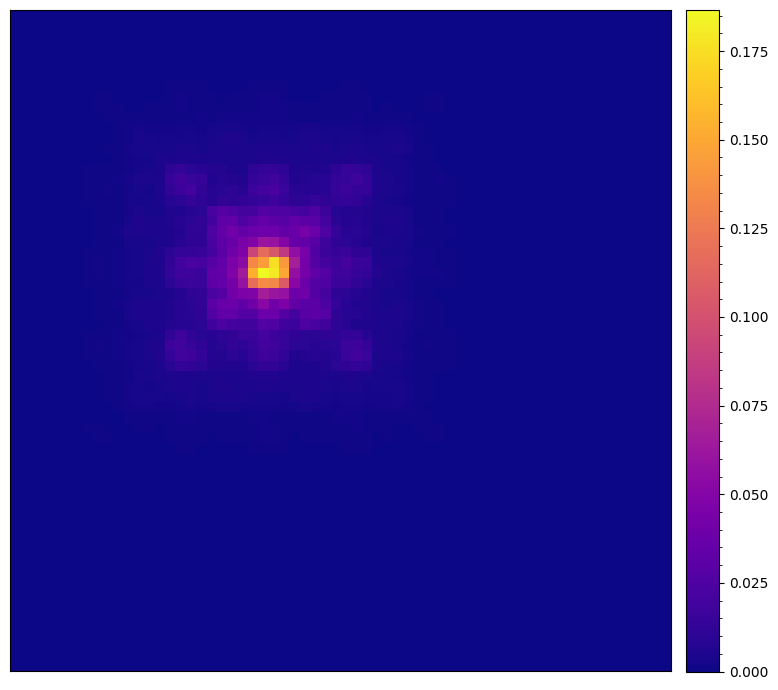
\includegraphics[width=0.7\textwidth]{images/gradientProjection_resnet_50_110.png}
%            \caption[Network1]%
%            {{\small Receptive field 110}}    
%            \label{fig:similarity_lvl1}
%        \end{subfigure}
%        \hfill
%        \begin{subfigure}[b]{0.475\textwidth}  
%            \centering 
%            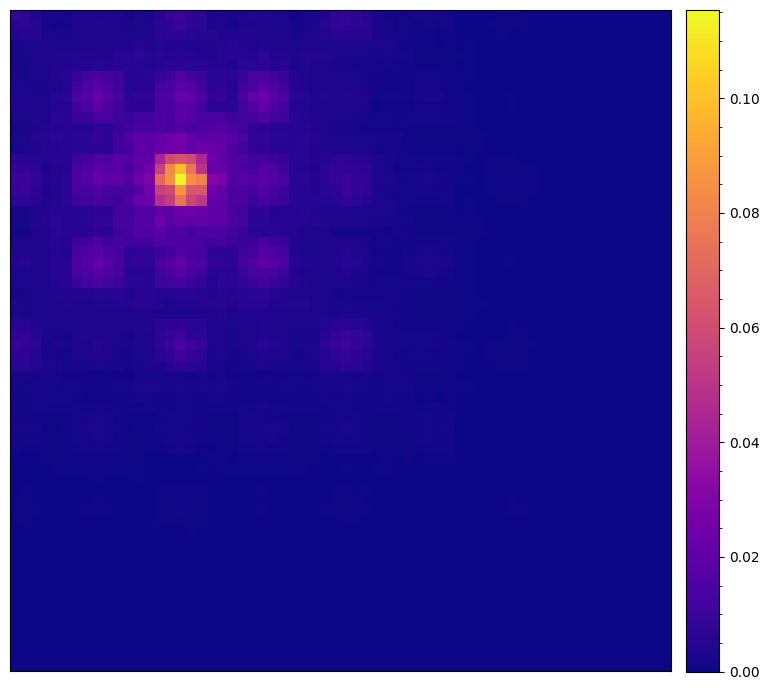
\includegraphics[width=0.7\textwidth]{images/gradientProjection_resnet_50_213.png}
%            \caption[Network2]%
%            {{\small Receptive field 213}}    
%            \label{fig:similarity_lvl2}
%        \end{subfigure}
%
%        \vskip\baselineskip
%
%        \begin{subfigure}[b]{0.475\textwidth}   
%            \centering 
%            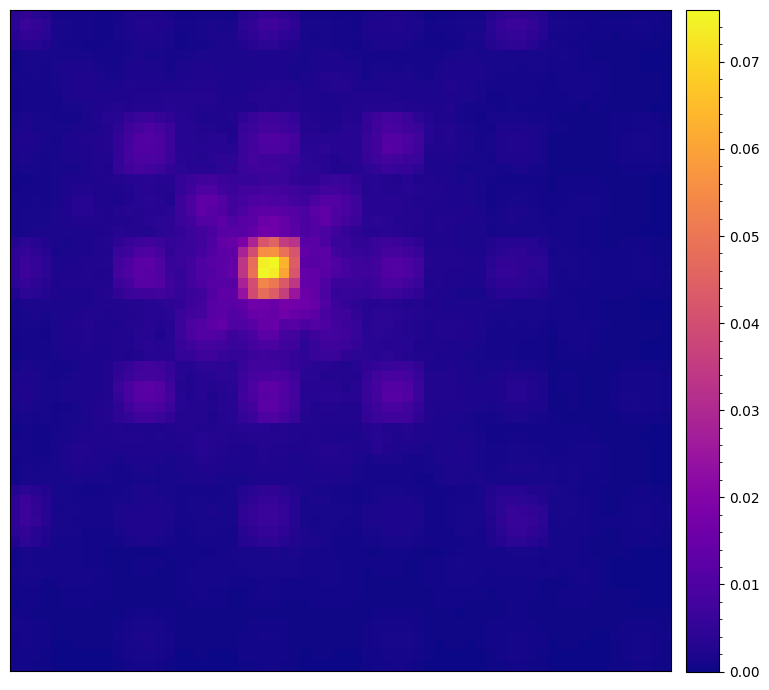
\includegraphics[width=0.7\textwidth]{images/gradientProjection_resnet_50_318.png}
%            \caption[]%
%            {{\small Receptive field 318}}    
%            \label{fig:similarity_lvl3}
%        \end{subfigure}
%        \hfill
%        \begin{subfigure}[b]{0.475\textwidth}   
%            \centering 
%            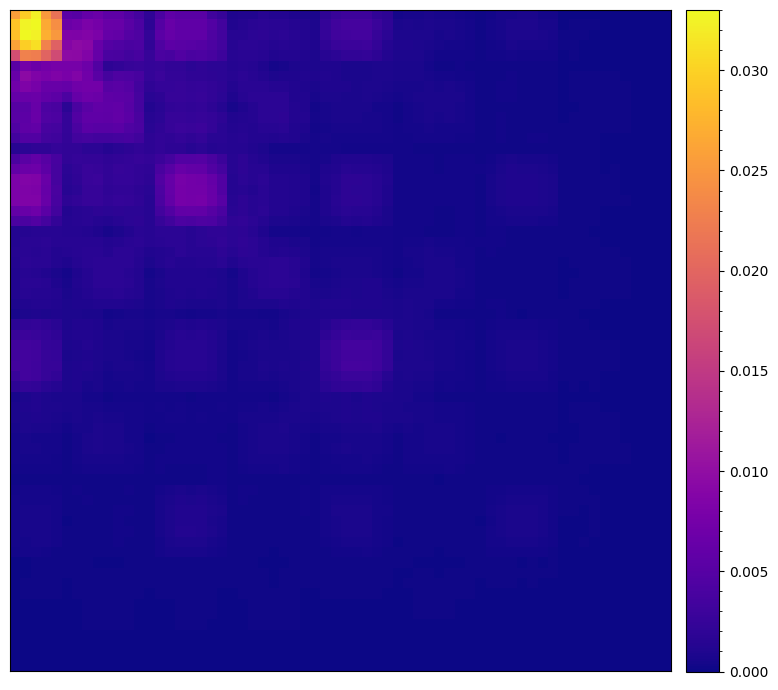
\includegraphics[width=0.7\textwidth]{images/gradientProjection_resnet_50_423.png}
%            \caption[]%
%            {{\small Receptive field 423}}    
%            \label{fig:similarity_lvl4}
%        \end{subfigure}
%        \caption{\small Projection of the gradient into an input space of 64x64 for different levels of receptive field
%        of ReseNet50}
%        \label{fig:gradient_projection_resenet50}
%    \end{figure}
%\begin{figure}[H]
%        \centering
%        \begin{subfigure}[b]{0.475\textwidth}
%            \centering
%            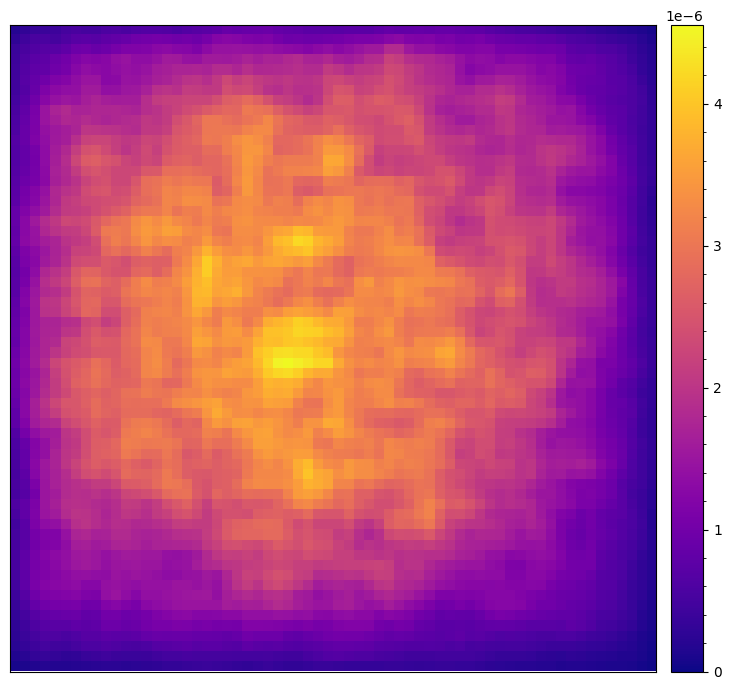
\includegraphics[width=0.7\textwidth]{images/gradientProjection_vgg19_1.png}
%            \caption[Network1]%
%            {{\small Receptive Field 181}}    
%            \label{fig:grad_projection_vgg_lvl1}
%        \end{subfigure}
%        \hfill
%        \begin{subfigure}[b]{0.475\textwidth}  
%            \centering 
%            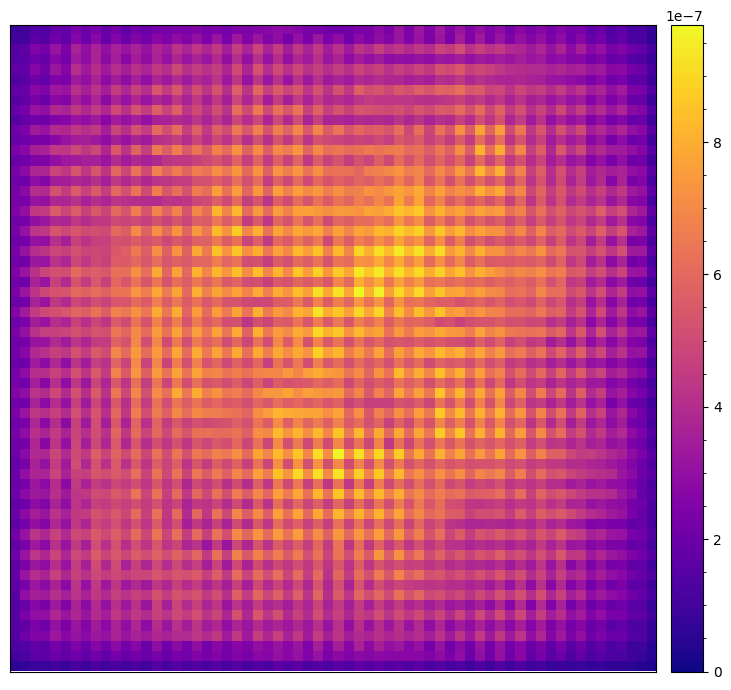
\includegraphics[width=0.7\textwidth]{images/gradientProjection_vgg19_2.png}
%            \caption[Network2]%
%            {{\small Receptive Field 359}}    
%            \label{fig:grad_projection_vgg_lvl2}
%        \end{subfigure}
%
%        \vskip\baselineskip
%
%        \begin{subfigure}[b]{0.475\textwidth}   
%            \centering 
%            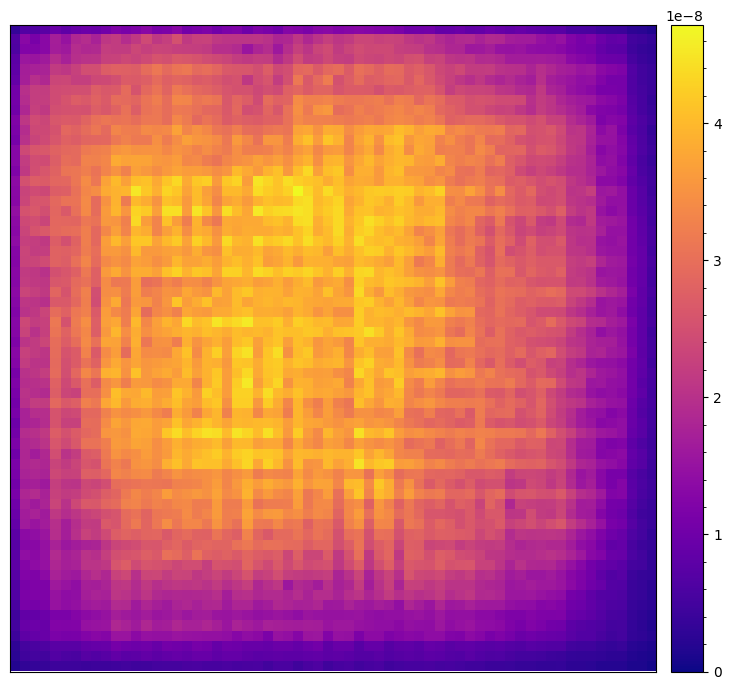
\includegraphics[width=0.7\textwidth]{images/gradientProjection_vgg19_3.png}
%            \caption[]%
%            {{\small Receptive Field 537}}    
%            \label{fig:grad_projection_vgg_lvl3}
%        \end{subfigure}
%        \hfill
%        \begin{subfigure}[b]{0.475\textwidth}   
%            \centering 
%            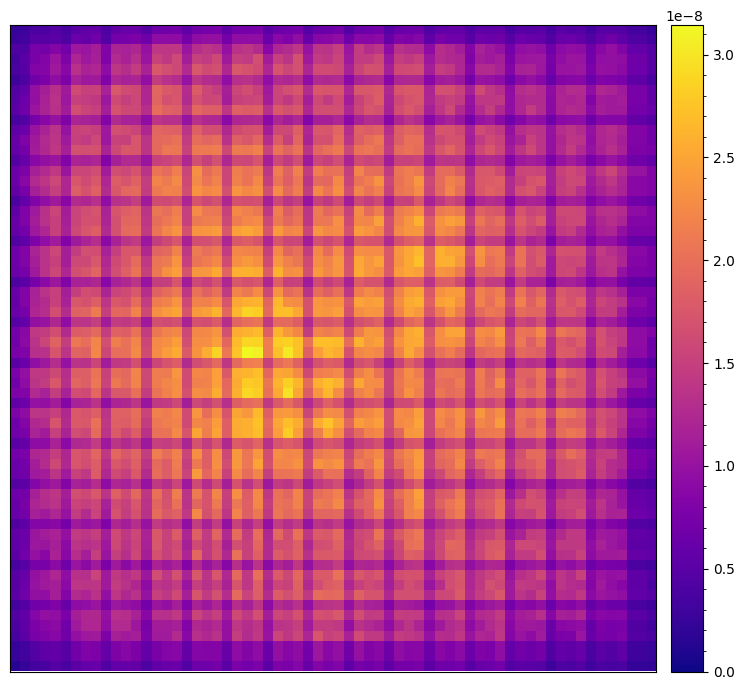
\includegraphics[width=0.7\textwidth]{images/gradientProjection_vgg19_4.png}
%            \caption[]%
%            {{\small Receptive Field 715}}    
%            \label{fig:grad_projection_vgg_lvl4}
%        \end{subfigure}
%        \caption{\small Projection of the gradient into an input space of 64x64 for different levels of receptive field
%        of ReseNet50}
%        \label{fig:gradient_projection_vgg}
%    \end{figure}
%
%
%
%\begin{table}[H]
%\begin{tabular}{@{}cc@{}}
%\toprule
%\textbf{Receptive Field} & \textbf{Maximum Projected Gradient Value} \\ \midrule
%181                      & 1.24e-05 $\pm$ 2.14e-06                   \\
%359                      & 2.48e-06 $\pm$ 4.88e-07                   \\
%537                      & 1.32e-07 $\pm$ 2.48e-08                   \\
%715                      & 7.26e-08 $\pm$ 1.45e-08                   \\ \bottomrule
%\end{tabular}
%\caption{VGG gradient projection on a 64X64 input image}
%\label{tab:vgg_grad_projection}
%\end{table}
%\begin{table}[H]
%\begin{tabular}{@{}cc@{}}
%\toprule
%\textbf{Receptive Field} & \textbf{Maximum Projected Gradient Value} \\ \midrule
%110                      & 0.322 $\pm$ 0.122                         \\
%213                      & 0.179 $\pm$ 0.079                         \\
%318                      & 0.111 $\pm$ 0.039                         \\
%423                      & 0.064 $\pm$ 0.022                         \\ \bottomrule
%\end{tabular}
%\caption{Maximum projected gradient for ReseNet50}
%\label{tab:resnet50_grad_projection}
%\end{table}
%
%
%\subsection{}
%
%
%
%\begin{figure*}[!htb]
% \centering
%     \begin{subfigure}[b]{\columnwidth}
%    \includegraphics[width=1.1\columnwidth]{}
%    \caption{}
%    \label{}
%     \end{subfigure}
%      \hfill
%     \begin{subfigure}[b]{\columnwidth}
%    \includegraphics[width=1.1\columnwidth]{}
%    \caption{}
%    \label{}
%     \end{subfigure}
%     \caption{}
%    \label{}
%\end{figure*}
%
%





%
%\begin{figure}[ht]
%  \centering
%  \includegraphics[width=0.8\textwidth]{}
%  \caption{}
%  \label{fig:}
%\end{figure}


\section{Conclusions and Future work}
\label{sec:conclusion}



 In this work, we showed how the receptive field affects the loss landscape of neural networks along with its representations and its behaviour on the input image.
It is important to note that there are other ways to manipulate the receptive field such as changing the kernel size of the
convolutional networks,stride, and dilation of the convolutional networks. In this work, used the minimum
intervention that would not modify the number of weights of the models as we manipulated the receptive field of the
models. Additionally, as we changed the receptive field of the models we changed the  size of internal representations,
which can greatly affect the behaviour of the models. Future work will concentrate on testing other ways to manipulate
the receptive field, such as dilation of the maxpooling layer, in addition to using padding to maintain constant the
size
of internal representations across receptive fields to test the robustness of the findings in this work.



%  References follow the acknowledgments in the camera-ready paper. Use unnumbered first-level heading for
%  the references. Any choice of citation style is acceptable as long as you are
%  consistent. It is permissible to reduce the font size to \verb+small+ (9 point)
%  when listing the references.
%  Note that the Reference section does not count towards the page limit.
  

  %\printbibliography
 % \nocite{*}

%  {
%  \small
%
%
%  [1] Alexander, J.A.\ \& Mozer, M.C.\ (1995) Template-based algorithms for
%  connectionist rule extraction. In G.\ Tesauro, D.S.\ Touretzky and T.K.\ Leen
%  (eds.), {\it Advances in Neural Information Processing Systems 7},
%  pp.\ 609--616. Cambridge, MA: MIT Press.
%
%
%  [2] Bower, J.M.\ \& Beeman, D.\ (1995) {\it The Book of GENESIS: Exploring
%    Realistic Neural Models with the GEneral NEural SImulation System.}  New York:
%  TELOS/Springer--Verlag.
%
%
%  [3] Hasselmo, M.E., Schnell, E.\ \& Barkai, E.\ (1995) Dynamics of learning and
%  recall at excitatory recurrent synapses and cholinergic modulation in rat
%  hippocampal region CA3. {\it Journal of Neuroscience} {\bf 15}(7):5249-5262.
%  }
%
  %%%%%%%%%%%%%%%%%%%%%%%%%%%%%%%%%%%%%%%%%%%%%%%%%%%%%%%%%%%%
  %                    REFERENCES                            %
  %%%%%%%%%%%%%%%%%%%%%%%%%%%%%%%%%%%%%%%%%%%%%%%%%%%%%%%%%%%%

  \bibliography{references.bib}




\beginsupplement
\section{Supplementary Material}
\label{sec:supplementary}

\subsection{Model Implementation details}
\label{sebsec:implementation_details}
Here are the implementation details.
\subsection*{One Shot solutions with multiple pruning rates}

\label{subsec:OneShotPruningrates}
For every combination 5 models were trained, pruned and fine-tuned. The error bars correspond to the standard deviation.
\todo[inline]{All of the following figures would be better on tables}
% Please add the following required packages to your document preamble:
% \usepackage{booktabs}
\begin{table}[]
\begin{tabular}{@{}cccc@{}}
\toprule
\multicolumn{4}{c}{\textbf{VGG}}                                                                                                                                  \\ \midrule
\textbf{Receptive Field} & \textbf{Dense Test Accuracy} & \multicolumn{1}{l}{\textbf{Pruned  TestAccuracy}} & \multicolumn{1}{l}{\textbf{Difference In Accuracy}} \\ \midrule
181                      & 93.52$\pm$0.115              & 72.22$\pm$27.11                                   & 21.30$\pm$27.18                                     \\
359                      & 91.15$\pm$0.232              & 90.23$\pm$1.32                                    & 0.916$\pm$1.50                                      \\
537                      & 87.87$\pm$0.193              & 87.87$\pm$0.193                                   & 0.0\textbackslash{}pm\$0.0                          \\
715                      & 85.88$\pm$0.217              & 85.880$\pm$0.217                                  & 0.0$\pm$0.0                                         \\ \midrule
\multicolumn{4}{c}{\textbf{ResNet50}}                                                                                                                             \\ \midrule
\textbf{Receptive Field} & \textbf{Dense Test Accuracy} & \textbf{Pruned  TestAccuracy}                     & \textbf{Difference In Accuracy}                     \\
110                      & 94.69$\pm$0.213              & 92.34$\pm$1.084                                   & 2.350$\pm$0.921                                     \\
213                      & 94.03$\pm$0.236              & 93.81$\pm$0.218                                   & 0.220$\pm$0.234                                     \\
318                      & 92.22$\pm$0.244              & 92.14$\pm$0.227                                   & 0.080$\pm$0.036                                     \\
423                      & 90.23$\pm$0.169              & 90.23$\pm$0.145                                   & -0.003$\pm$0.035                                    \\ \bottomrule
\end{tabular}



\caption{vgg and resent50 cifar10 pruning rate 0.8}
\label{tab:cifar10 pruning rate08}
\end{table}

% Please add the following required packages to your document preamble:
% \usepackage{booktabs}
\begin{table}[]
\begin{tabular}{@{}cccc@{}}
\toprule
\multicolumn{4}{c}{\textbf{VGG}}                                                                                                                                  \\ \midrule
\textbf{Receptive Field} & \textbf{Dense Test Accuracy} & \multicolumn{1}{l}{\textbf{Pruned  TestAccuracy}} & \multicolumn{1}{l}{\textbf{Difference In Accuracy}} \\ \midrule
181                      & 61.58$\pm$0.333              & 19.14$\pm$4.610                                   & 42.44$\pm$4.669                                     \\
359                      & 53.25$\pm$0.207              & 10.09$\pm$1.931                                   & 43.16$\pm$2.085                                     \\
537                      & 41.05$\pm$1.917              & 40.09$\pm$2.129                                   & 0.958$\pm$0.360                                     \\
715                      & 38.57$\pm$1.691              & 37.87$\pm$1.566                                   & 0.700$\pm$0.524                                     \\ \midrule
\multicolumn{4}{c}{\textbf{ResNet50}}                                                                                                                             \\ \midrule
\textbf{Receptive Field} & \textbf{Dense Test Accuracy} & \textbf{Pruned  TestAccuracy}                     & \textbf{Difference In Accuracy}                     \\
213                      & 61.83$\pm$0.401              & 40.56$\pm$3.039                                   & 21.27$\pm$3.170                                     \\
318                      & 59.10$\pm$0.368              & 43.09$\pm$1.880                                   & 16.01$\pm$1.824                                     \\
423                      & 56.53$\pm$0.279              & 49.27$\pm$0.580                                   & 7.260$\pm$0.412                                     \\ \bottomrule
\end{tabular}
\caption{vgg and resent50 tiny Image net pruning rate 0.8}
\label{tab:tiny imagenet pruning rate08}
\end{table}


%
%\begin{figure}[h]
% \centering
%     \begin{subfigure}[b]{\columnwidth}
%    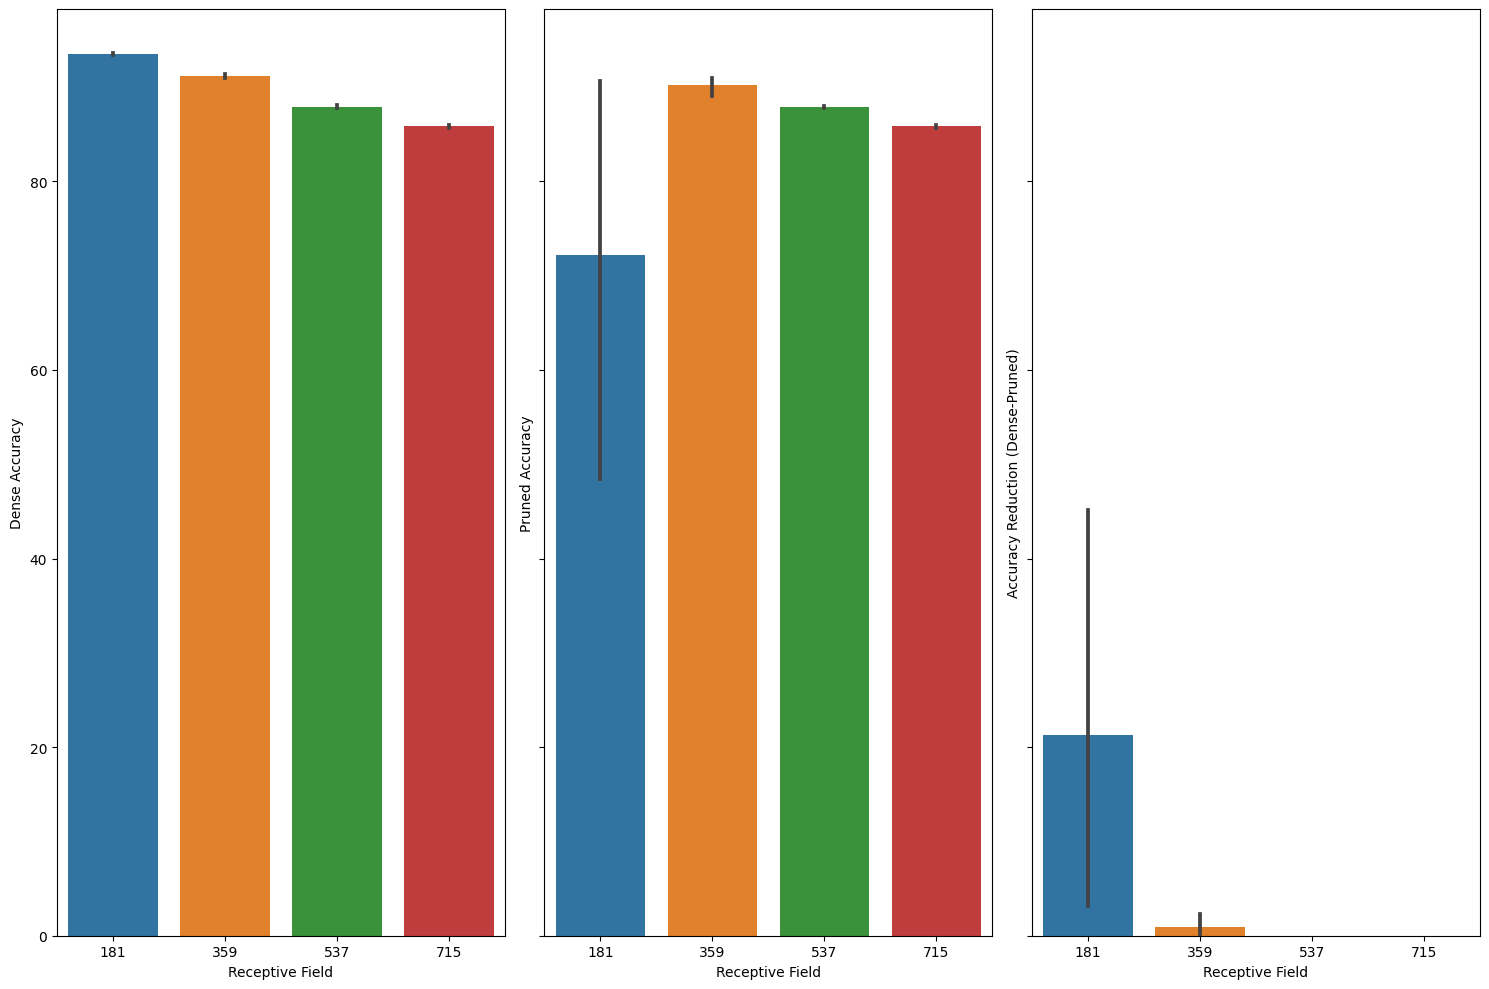
\includegraphics[width=1.1\columnwidth]{images/Supplementary_material/cifar10_vgg19_pruning_results_0.8.png}
%    \caption{VGG}
%    \label{subfig:vgg19CIfar10PR0.8}
%     \end{subfigure}
%      \hfill
%     \begin{subfigure}[b]{\columnwidth}
%    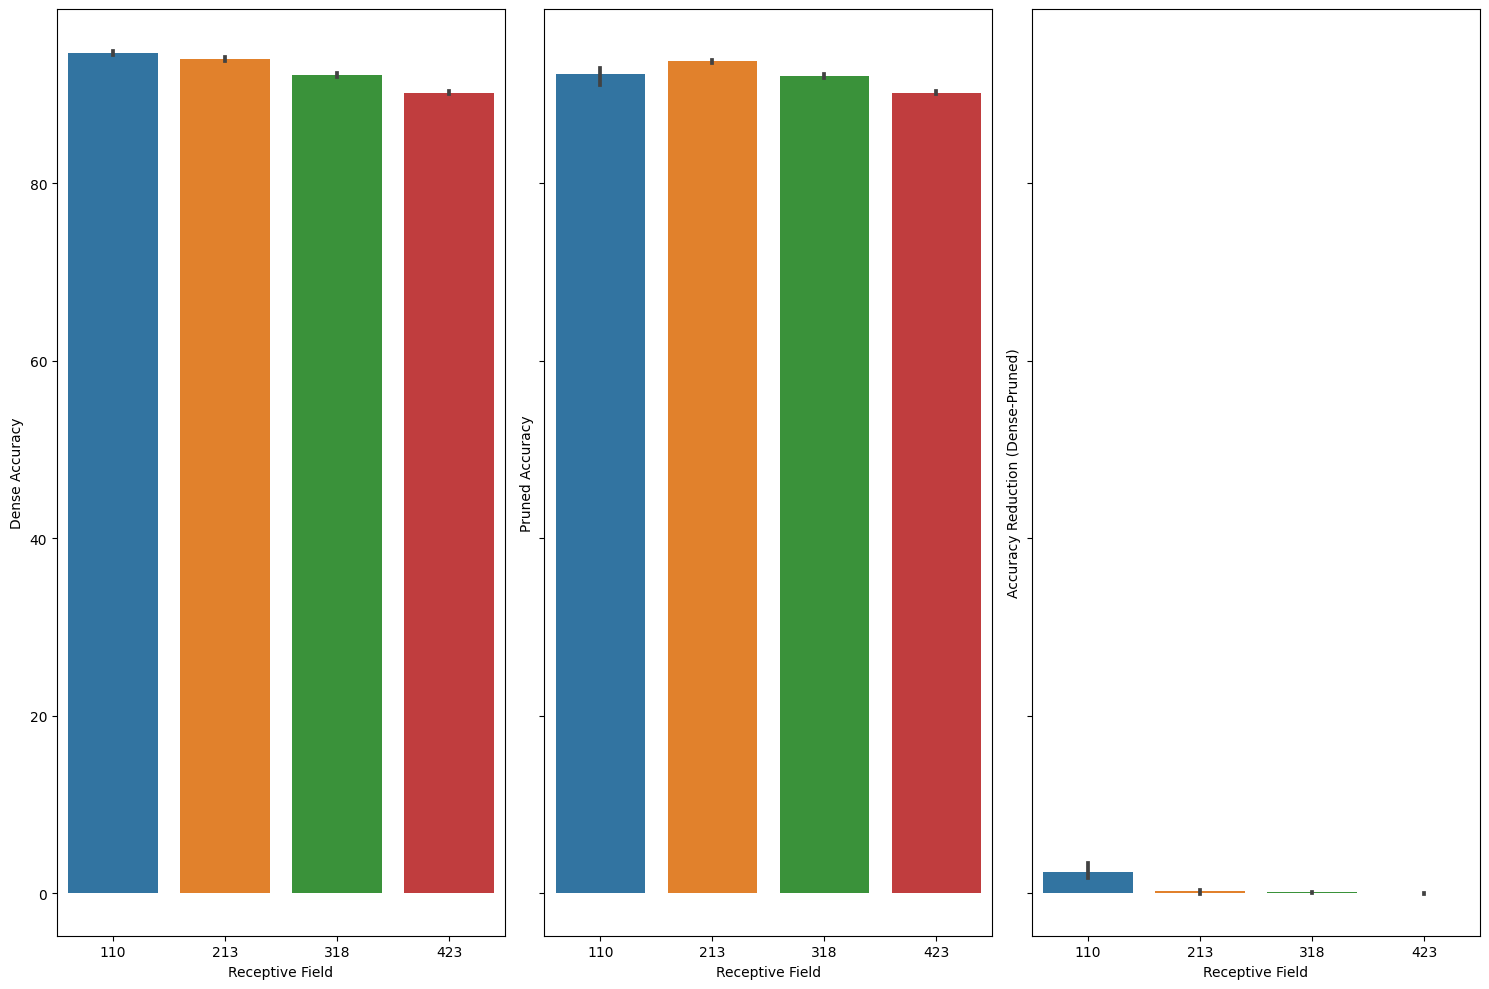
\includegraphics[width=1.1\columnwidth]{images/Supplementary_material/cifar10_resnet50_pruning_results_0.8.png}
%    \caption{ResNet-50}
%    \label{subfig:resenet50CIfar10PR0.8}
%     \end{subfigure}
%     \caption{ CIFAR10 pruning rate 0.8 results}
%    \label{fig:pr_0.8_CIFAR10}
%\end{figure}
%
%\begin{figure}[h]
% \centering
%     \begin{subfigure}[b]{\columnwidth}
%    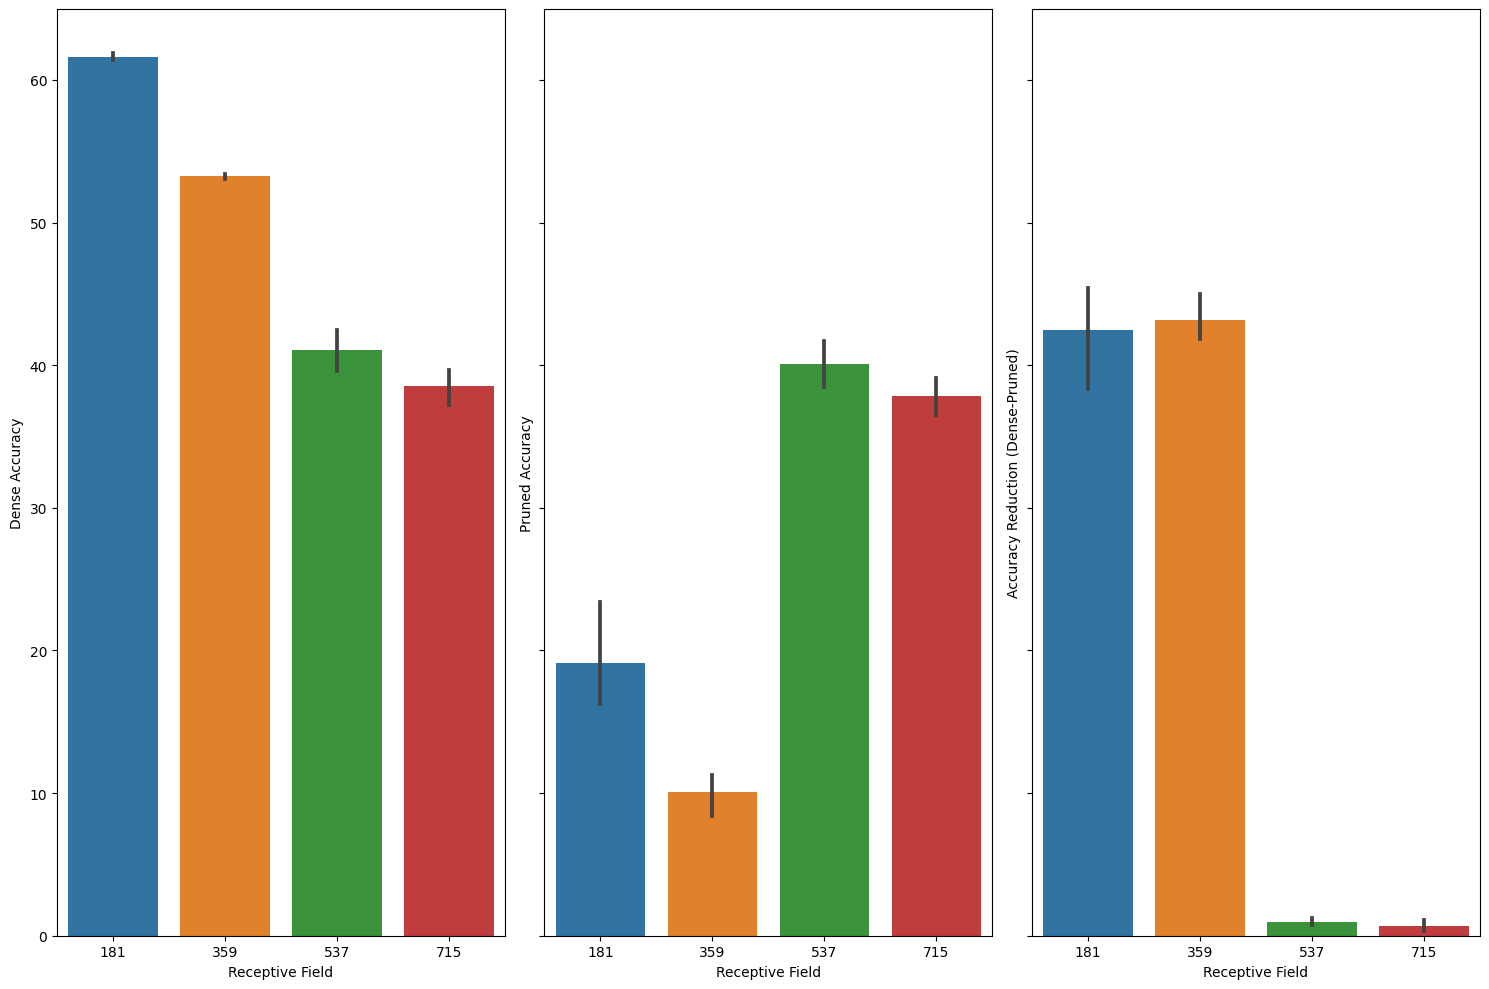
\includegraphics[width=1.1\columnwidth]{images/Supplementary_material/tiny_imagenet_vgg19_pruning_results_0.8.png}
%    \caption{VGG}
%    \label{subfig:vgg19CIfar10PR0.8}
%     \end{subfigure}
%      \hfill
%     \begin{subfigure}[b]{\columnwidth}
%    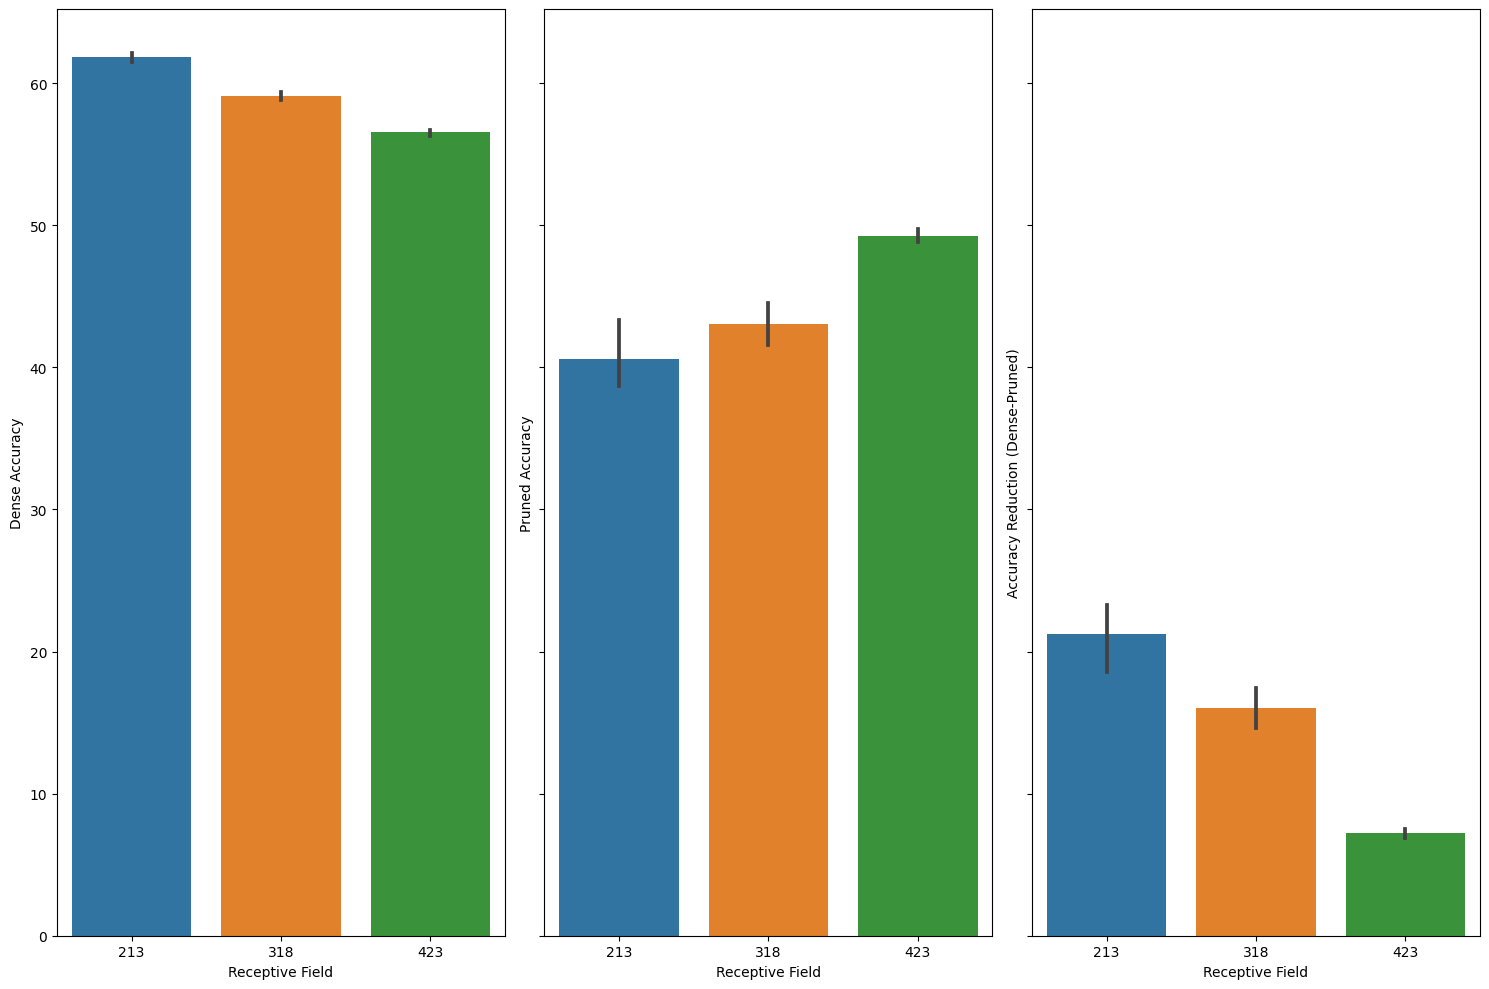
\includegraphics[width=1.1\columnwidth]{images/Supplementary_material/tiny_imagenet_resnet50_pruning_results_0.8.png}
%    \caption{ResNet-50}
%    \label{subfig:resenet50CIfar10PR0.8}
%     \end{subfigure}
%     \caption{ Tiny ImageNet pruning 0.8 results}
%    \label{fig:pr_0.8_tiny_imagenet}
%\end{figure}
%
\subsubsection*{Pruning rate 0.7}
% Please add the following required packages to your document preamble:
% \usepackage{booktabs}
\begin{table}[]
\begin{tabular}{@{}cccc@{}}
\toprule
\multicolumn{4}{c}{\textbf{VGG}}                                                                                                                                  \\ \midrule
\textbf{Receptive Field} & \textbf{Dense Test Accuracy} & \multicolumn{1}{l}{\textbf{Pruned  TestAccuracy}} & \multicolumn{1}{l}{\textbf{Difference In Accuracy}} \\ \midrule
181                      & 93.52$\pm$0.115              & 93.32$\pm$0.104                                   & 0.206$\pm$0.155                                     \\
359                      & 91.15$\pm$0.232              & 91.10$\pm$0.230                                   & 0.058$\pm$0.050                                     \\
537                      & 87.88$\pm$0.193              & 87.88$\pm$0.193                                   & 0.0$\pm$0.0                                         \\
715                      & 85.88$\pm$0.217              & 85.88$\pm$0.217                                   & 0.0$\pm$0.0                                         \\ \midrule
\multicolumn{4}{c}{\textbf{ResNet50}}                                                                                                                             \\ \midrule
\textbf{Receptive Field} & \textbf{Dense Test Accuracy} & \textbf{Pruned  TestAccuracy}                     & \textbf{Difference In Accuracy}                     \\
110                      & 94.69$\pm$0.213              & 94.24$\pm$0.204                                   & 0.453$\pm$0.012                                     \\
213                      & 94.03$\pm$0.236              & 93.93$\pm$0.203                                   & 0.097$\pm$0.093                                     \\
318                      & 92.22$\pm$0.244              & 92.24$\pm$0.254                                   & -0.020$\pm$0.010                                    \\
423                      & 90.23$\pm$0.169              & 90.23$\pm$0.175                                   & -0.007$\pm$0.006                                    \\ \bottomrule
\end{tabular}
\caption{vgg and resent50 cifar10 pruning rate 0.7}
\label{tab:cifar10 pruning rate07}
\end{table}
% Please add the following required packages to your document preamble:
% \usepackage{booktabs}
\begin{table}[]
\begin{tabular}{@{}cccc@{}}
\toprule
\multicolumn{4}{c}{\textbf{VGG}}                                                                                                                                  \\ \midrule
\textbf{Receptive Field} & \textbf{Dense Test Accuracy} & \multicolumn{1}{l}{\textbf{Pruned  TestAccuracy}} & \multicolumn{1}{l}{\textbf{Difference In Accuracy}} \\ \midrule
181                      & 61.58$\pm$0.333              & 48.29$\pm$1.390                                   & 13.29$\pm$1.462                                     \\
359                      & 53.25$\pm$0.207              & 40.02$\pm$2.558                                   & 13.23$\pm$2.646                                     \\
537                      & 41.05$\pm$1.917              & 40.96$\pm$1.934                                   & 0.092$\pm$0.070                                     \\
715                      & 38.57$\pm$1.691              & 38.51$\pm$1.658                                   & 0.068$\pm$0.087                                     \\ \midrule
\multicolumn{4}{c}{\textbf{ResNet50}}                                                                                                                             \\ \midrule
\textbf{Receptive Field} & \textbf{Dense Test Accuracy} & \textbf{Pruned  TestAccuracy}                     & \textbf{Difference In Accuracy}                     \\
213                      & 61.83$\pm$0.401              & 55.33$\pm$0.987                                   & 6.504$\pm$1.194                                     \\
318                      & 59.10$\pm$0.368              & 54.28$\pm$0.398                                   & 4.816$\pm$0.319                                     \\
423                      & 56.53$\pm$0.279              & 54.41$\pm$0.449                                   & 2.128$\pm$0.216                                     \\ \bottomrule
\end{tabular}
\caption{vgg and resent50 tiny Image net pruning rate 0.7}
\label{tab:tiny imagenet pruning rate07}
\end{table}
%
%\begin{figure}[h]
% \centering
%     \begin{subfigure}[b]{\columnwidth}
%    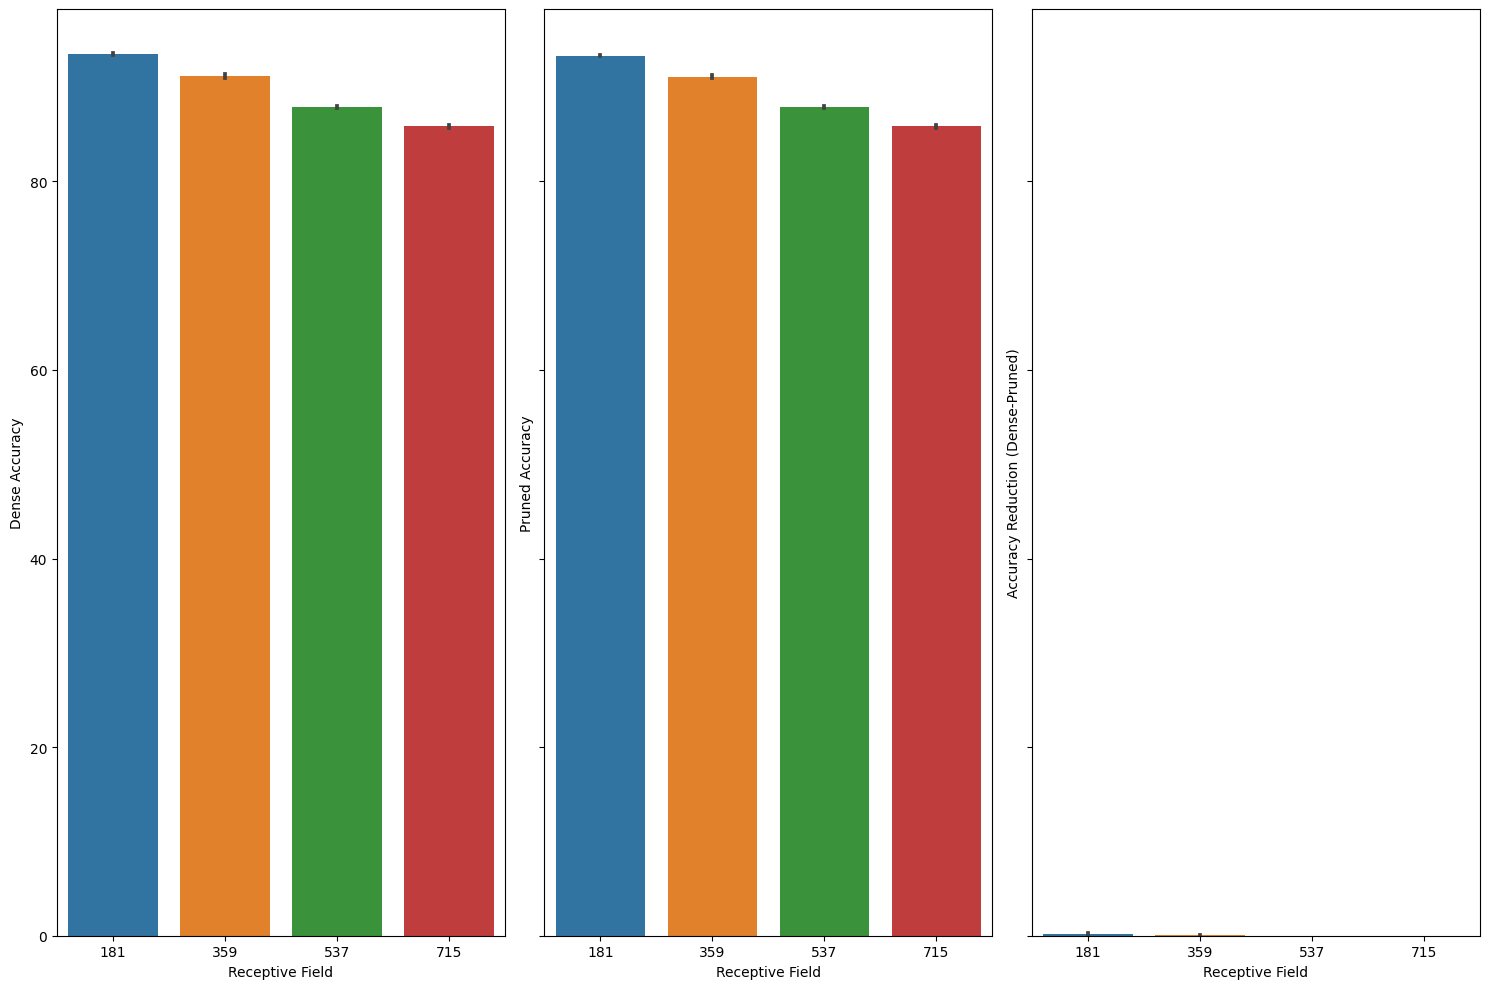
\includegraphics[width=1.1\columnwidth]{images/Supplementary_material/cifar10_vgg19_pruning_results_0.7.png}
%    \caption{VGG}
%    \label{subfig:vgg19CIfar10PR0.7}
%     \end{subfigure}
%      \hfill
%     \begin{subfigure}[b]{\columnwidth}
%    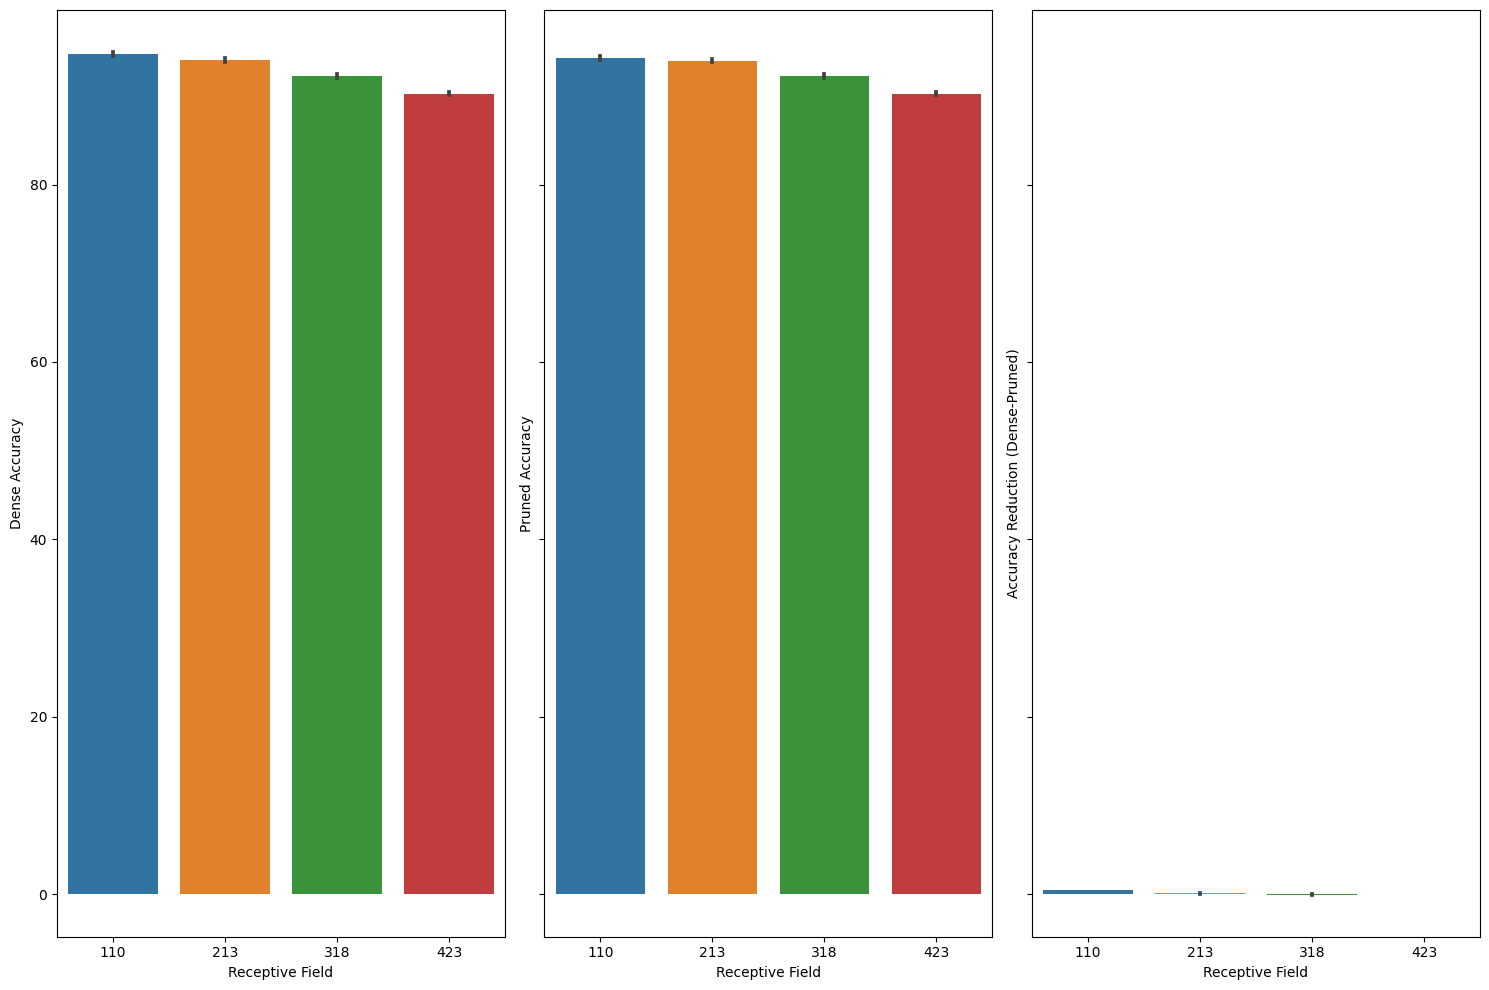
\includegraphics[width=1.1\columnwidth]{images/Supplementary_material/cifar10_resnet50_pruning_results_0.7.png}
%    \caption{ResNet-50}
%    \label{subfig:resenet50CIfar10PR0.7}
%     \end{subfigure}
%     \caption{ CIFAR10 0.7 results}
%    \label{fig:pr_0.7_CIFAR10}
%\end{figure}
%
%
%\begin{figure}[h]
% \centering
%     \begin{subfigure}[b]{\columnwidth}
%    \includegraphics[width=1.1\columnwidth]{images/Supplementary_material/tiny_imagenet_vgg19_pruning_results_0.7.png}
%    \caption{VGG}
%    \label{subfig:vgg19CIfar10PR0.7}
%     \end{subfigure}
%      \hfill
%     \begin{subfigure}[b]{\columnwidth}
%    \includegraphics[width=1.1\columnwidth]{images/Supplementary_material/tiny_imagenet_resnet50_pruning_results_0.7.png}
%    \caption{ResNet-50}
%    \label{subfig:resenet50CIfar10PR0.7}
%     \end{subfigure}
%     \caption{ Tiny ImageNet pruning 0.7 results}
%    \label{fig:pr_0.7_tiny_imagenet}
%\end{figure}
%
%
\subsubsection*{Pruning rate 0.6}

% Please add the following required packages to your document preamble:
% \usepackage{booktabs}
\begin{table}[]
\begin{tabular}{@{}cccc@{}}
\toprule
\multicolumn{4}{c}{\textbf{VGG}}                                                                                                                                  \\ \midrule
\textbf{Receptive Field} & \textbf{Dense Test Accuracy} & \multicolumn{1}{l}{\textbf{Pruned  TestAccuracy}} & \multicolumn{1}{l}{\textbf{Difference In Accuracy}} \\ \midrule
181                      & 93.52$\pm$0.115              & 93.48$\pm$0.109                                   & 0.048$\pm$0.050                                     \\
359                      & 91.15$\pm$0.232              & 91.15$\pm$0.240                                   & 0.004$\pm$0.015                                     \\
537                      & 87.88$\pm$0.193              & 87.88$\pm$0.193                                   & 0.000$\pm$0.000                                     \\
715                      & 85.88$\pm$0.217              & 85.88$\pm$0.217                                   & 0.000$\pm$0.000                                     \\ \midrule
\multicolumn{4}{c}{\textbf{ResNet50}}                                                                                                                             \\ \midrule
\textbf{Receptive Field} & \textbf{Dense Test Accuracy} & \textbf{Pruned  TestAccuracy}                     & \textbf{Difference In Accuracy}                     \\
110                      & 94.69$\pm$0.213              & 94.61$\pm$0.190                                   & 0.080$\pm$0.026                                     \\
213                      & 94.03$\pm$0.236              & 94.01$\pm$0.234                                   & 0.020$\pm$0.020                                     \\
318                      & 92.22$\pm$0.244              & 92.23$\pm$0.225                                   & -0.010$\pm$0.020                                    \\
423                      & 90.23$\pm$0.169              & 90.23$\pm$0.169                                   & 0.000$\pm$0.000                                     \\ \bottomrule
\end{tabular}
\caption{vgg and resent50 cifar10 pruning rate 0.6}
\label{tab:cifar10 pruning rate06}
\end{table}




% Please add the following required packages to your document preamble:
% \usepackage{booktabs}
\begin{table}[]
\begin{tabular}{@{}cccc@{}}
\toprule
\multicolumn{4}{c}{\textbf{VGG}}                                                                                                                                  \\ \midrule
\textbf{Receptive Field} & \textbf{Dense Test Accuracy} & \multicolumn{1}{l}{\textbf{Pruned  TestAccuracy}} & \multicolumn{1}{l}{\textbf{Difference In Accuracy}} \\ \midrule
181                      & 61.58$\pm$0.333              & 56.93$\pm$0.512                                   & 4.656$\pm$0.663                                     \\
359                      & 53.25$\pm$0.207              & 47.94$\pm$1.896                                   & 5.304$\pm$1.963                                     \\
537                      & 41.05$\pm$1.917              & 41.05$\pm$1.913                                   & -0.000$\pm$0.071                                    \\
715                      & 38.57$\pm$1.691              & 38.58$\pm$1.659                                   & -0.008$\pm$0.039                                    \\ \midrule
\multicolumn{4}{c}{\textbf{ResNet50}}                                                                                                                             \\ \midrule
\textbf{Receptive Field} & \textbf{Dense Test Accuracy} & \textbf{Pruned  TestAccuracy}                     & \textbf{Difference In Accuracy}                     \\
213                      & 61.83$\pm$0.401              & 59.28$\pm$0.468                                   & 2.552$\pm$0.489                                     \\
318                      & 59.10$\pm$0.368              & 57.26$\pm$0.467                                   & 1.840$\pm$0.356                                     \\
423                      & 56.53$\pm$0.279              & 55.97$\pm$0.459                                   & 0.568$\pm$0.212                                     \\ \bottomrule
\end{tabular}
\caption{vgg and resent50 tiny Image net pruning rate 0.6}
\label{tab:tiny imagenet pruning rate06}
\end{table}




%
%\begin{figure}[h]
% \centering
%     \begin{subfigure}[b]{\columnwidth}
%    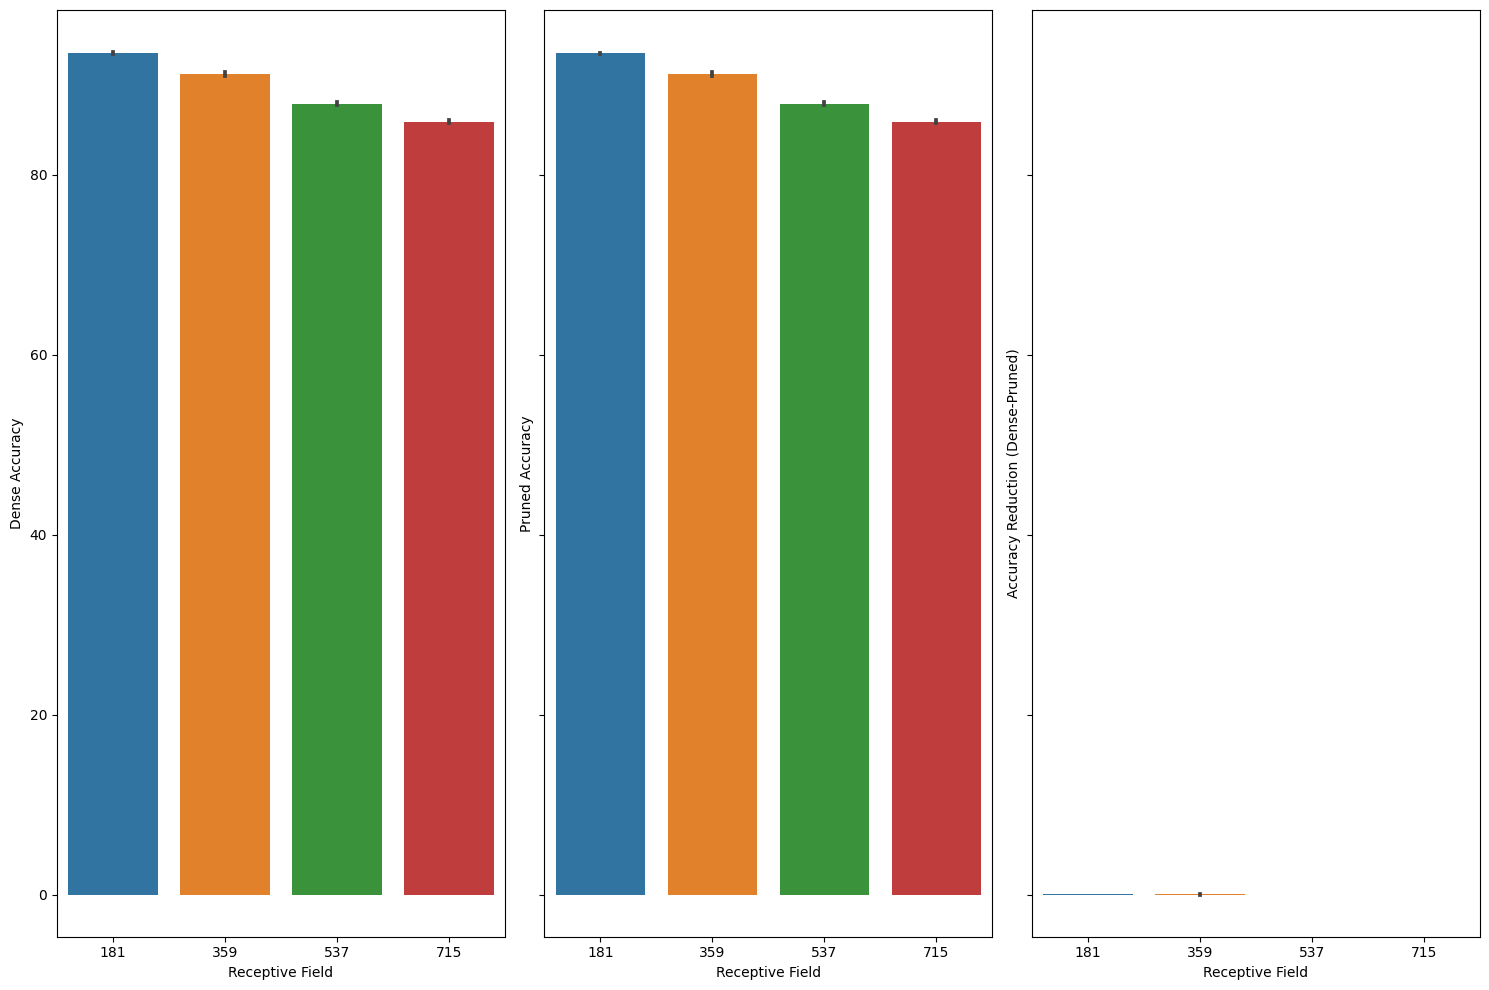
\includegraphics[width=1.1\columnwidth]{images/Supplementary_material/cifar10_vgg19_pruning_results_0.6.png}
%    \caption{VGG}
%    \label{subfig:vgg19CIfar10PR0.6}
%     \end{subfigure}
%      \hfill
%     \begin{subfigure}[b]{\columnwidth}
%    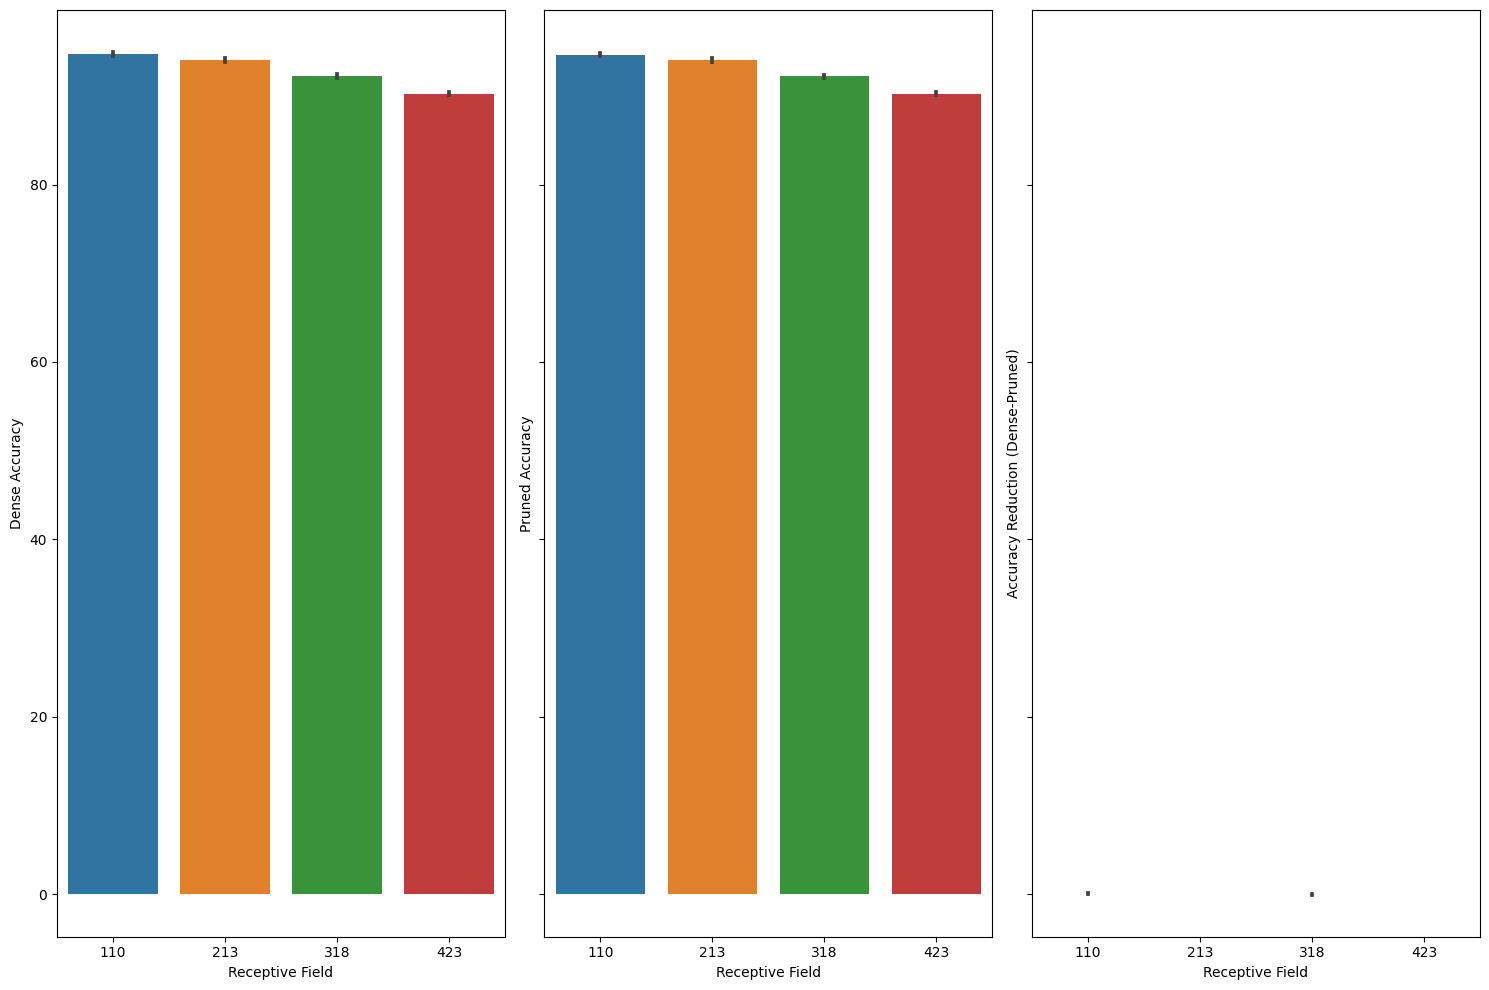
\includegraphics[width=1.1\columnwidth]{images/Supplementary_material/cifar10_resnet50_pruning_results_0.6.png}
%    \caption{ResNet-50}
%    \label{subfig:resenet50CIfar10PR0.6}
%     \end{subfigure}
%     \caption{ CIFAR10 0.6 results}
%    \label{fig:pr_0.7_CIFAR10}
%\end{figure}
%
%
%\begin{figure}[h]
% \centering
%     \begin{subfigure}[b]{\columnwidth}
%    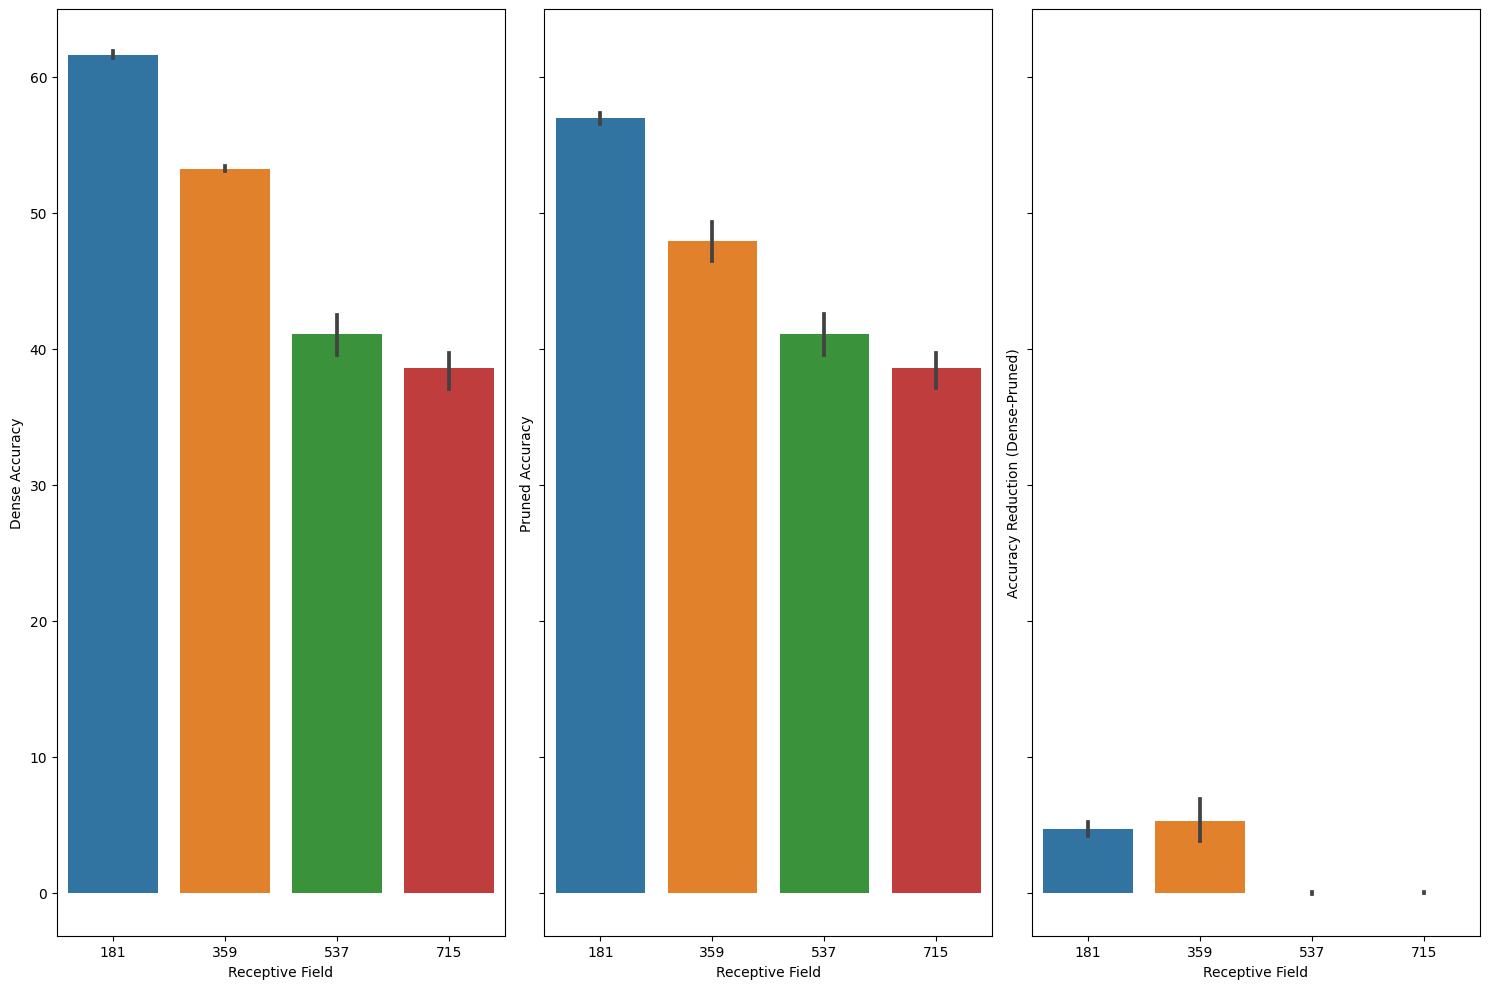
\includegraphics[width=1.1\columnwidth]{images/Supplementary_material/tiny_imagenet_vgg19_pruning_results_0.6.png}
%    \caption{VGG}
%    \label{subfig:vgg19CIfar10PR0.6}
%     \end{subfigure}
%      \hfill
%     \begin{subfigure}[b]{\columnwidth}
%    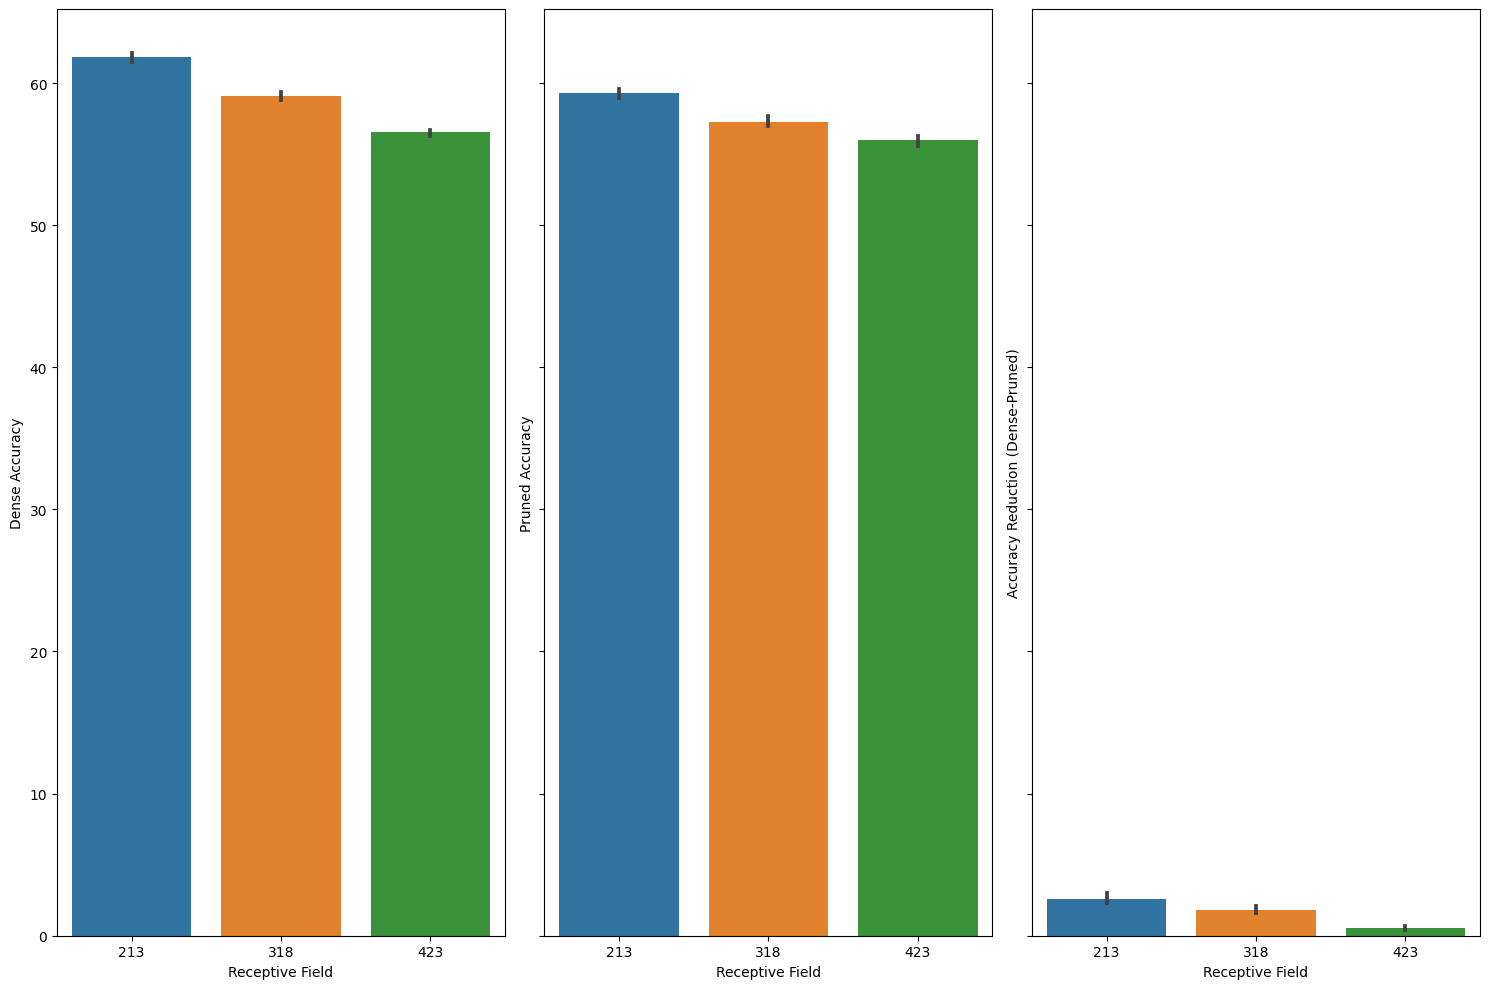
\includegraphics[width=1.1\columnwidth]{images/Supplementary_material/tiny_imagenet_resnet50_pruning_results_0.6.png}
%    \caption{ResNet-50}
%    \label{subfig:resenet50CIfar10PR0.6}
%     \end{subfigure}
%     \caption{ Tiny ImageNet 0.6 results}
%
%    \label{fig:pr_0.6_tiny_imagenet}
%
%\end{figure}
%
\subsubsection*{Pruning rate 0.5}
% Please add the following required packages to your document preamble:
% \usepackage{booktabs}
\begin{table}[]
\begin{tabular}{@{}cccc@{}}
\toprule
\multicolumn{4}{c}{\textbf{VGG}}                                                                                                                                  \\ \midrule
\textbf{Receptive Field} & \textbf{Dense Test Accuracy} & \multicolumn{1}{l}{\textbf{Pruned  TestAccuracy}} & \multicolumn{1}{l}{\textbf{Difference In Accuracy}} \\ \midrule
181                      & 93.52$\pm$0.115              & 93.51$\pm$0.128                                   & 0.010$\pm$0.029                                     \\
359                      & 91.15$\pm$0.232              & 91.16$\pm$0.237                                   & -0.004$\pm$0.005                                    \\
537                      & 87.88$\pm$0.193              & 87.88$\pm$0.193                                   & 0.000$\pm$0.000                                     \\
715                      & 85.88$\pm$0.217              & 85.88$\pm$0.217                                   & 0.000$\pm$0.000                                     \\ \midrule
\multicolumn{4}{c}{\textbf{ResNet50}}                                                                                                                             \\ \midrule
\textbf{Receptive Field} & \textbf{Dense Test Accuracy} & \textbf{Pruned  TestAccuracy}                     & \textbf{Difference In Accuracy}                     \\
110                      & 94.69$\pm$0.213              & 94.71$\pm$0.202                                   & -0.023$\pm$0.012                                    \\
213                      & 94.03$\pm$0.236              & 94.02$\pm$0.243                                   & 0.010$\pm$0.026                                     \\
318                      & 92.22$\pm$0.244              & 92.22$\pm$0.229                                   & -0.003$\pm$0.015                                    \\
423                      & 90.23$\pm$0.169              & 90.23$\pm$0.169                                   & 0.000$\pm$0.000                                     \\ \bottomrule
\end{tabular}
\caption{vgg and resent50 cifar10 pruning rate 0.5}
\label{tab:cifar10 pruning rate05}
\end{table}
% Please add the following required packages to your document preamble:
% \usepackage{booktabs}
\begin{table}[]
\begin{tabular}{@{}cccc@{}}
\toprule
\multicolumn{4}{c}{\textbf{VGG}}                                                                                                                                  \\ \midrule
\textbf{Receptive Field} & \textbf{Dense Test Accuracy} & \multicolumn{1}{l}{\textbf{Pruned  TestAccuracy}} & \multicolumn{1}{l}{\textbf{Difference In Accuracy}} \\ \midrule
181                      & 61.58$\pm$0.333              & 59.85$\pm$0.241                                   & 1.738$\pm$0.240                                     \\
359                      & 53.25$\pm$0.207              & 51.13$\pm$0.665                                   & 2.116$\pm$0.735                                     \\
537                      & 41.05$\pm$1.917              & 41.05$\pm$1.915                                   & -0.004$\pm$0.018                                    \\
715                      & 38.57$\pm$1.691              & 38.57$\pm$1.686                                   & 0.008$\pm$0.013                                     \\ \midrule
\multicolumn{4}{c}{\textbf{ResNet50}}                                                                                                                             \\ \midrule
\textbf{Receptive Field} & \textbf{Dense Test Accuracy} & \textbf{Pruned  TestAccuracy}                     & \textbf{Difference In Accuracy}                     \\
213                      & 61.83$\pm$0.401              & 60.86$\pm$0.458                                   & 0.966$\pm$0.400                                     \\
318                      & 59.10$\pm$0.368              & 58.46$\pm$0.510                                   & 0.640$\pm$0.401                                     \\
423                      & 56.53$\pm$0.279              & 56.29$\pm$0.408                                   & 0.248$\pm$0.180                                     \\ \bottomrule
\end{tabular}
\caption{vgg and resent50 tiny Image net pruning rate 0.5}
\label{tab:tiny imagenet pruning rate06}
\end{table}

%
%\begin{figure}[h]
% \centering
%     \begin{subfigure}[b]{\columnwidth}
%    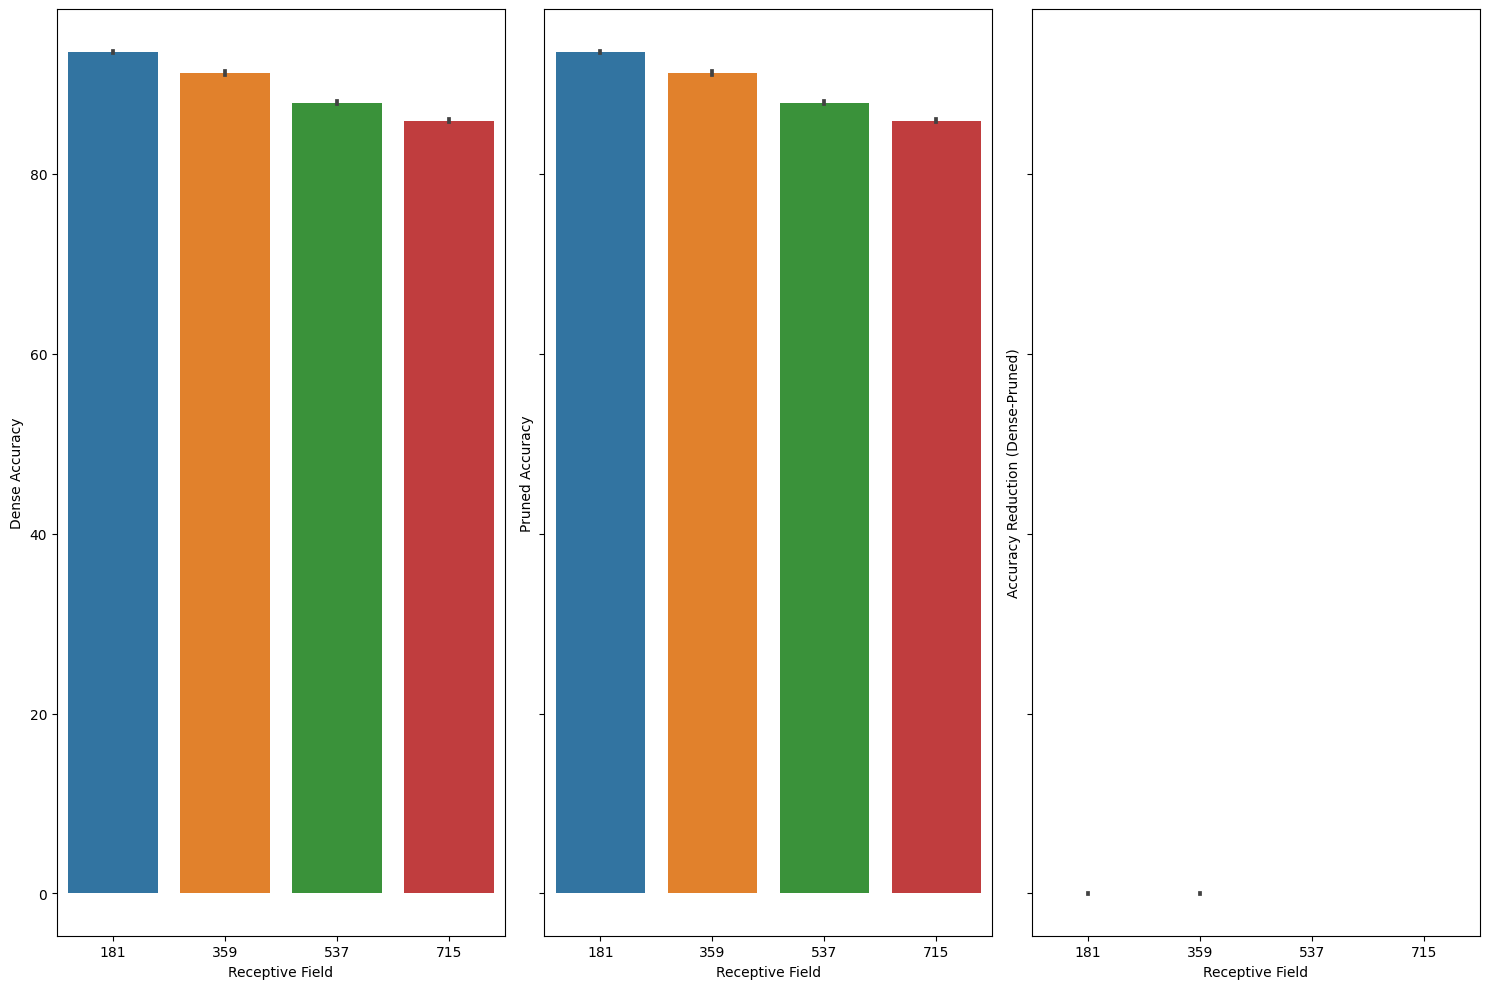
\includegraphics[width=1.1\columnwidth]{images/Supplementary_material/cifar10_vgg19_pruning_results_0.5.png}
%    \caption{VGG}
%    \label{subfig:vgg19CIfar10PR0.5}
%     \end{subfigure}
%      \hfill
%     \begin{subfigure}[b]{\columnwidth}
%    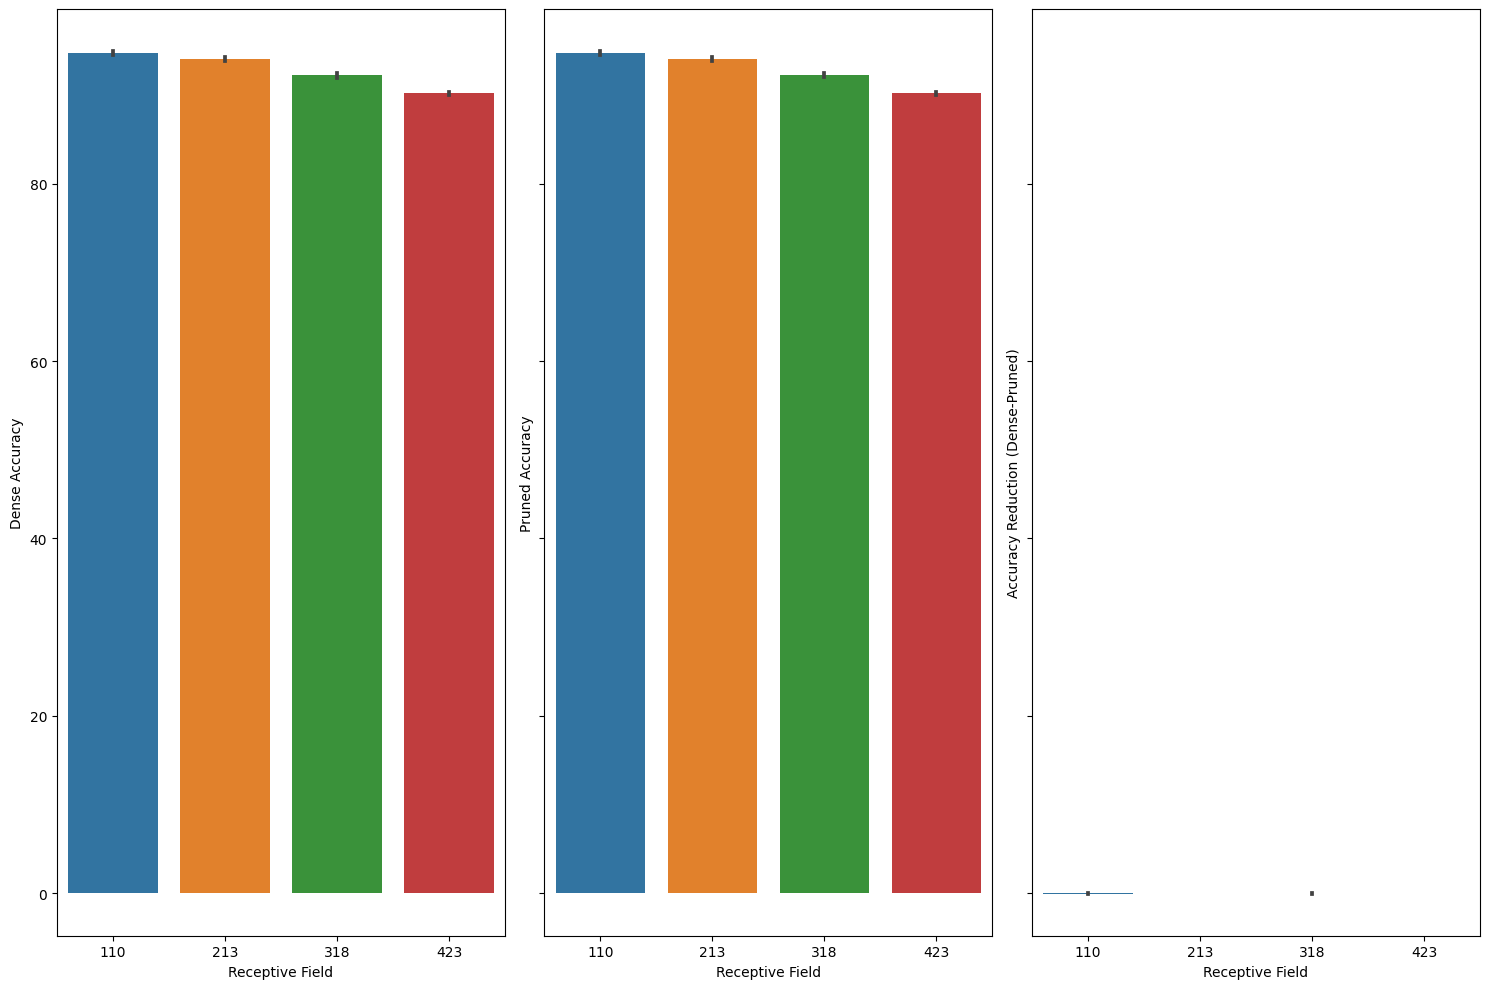
\includegraphics[width=1.1\columnwidth]{images/Supplementary_material/cifar10_resnet50_pruning_results_0.5.png}
%    \caption{ResNet-50}
%    \label{subfig:resenet50CIfar10PR0.5}
%     \end{subfigure}
%     \caption{ CIFAR10 0.5 results}
%    \label{fig:pr_0.5_CIFAR10}
%\end{figure}
%
%
%\begin{figure}[h]
% \centering
%     \begin{subfigure}[b]{\columnwidth}
%    \includegraphics[width=1.1\columnwidth]{images/Supplementary_material/tiny_imagenet_vgg19_pruning_results_0.5.png}
%    \caption{VGG}
%    \label{subfig:vgg19CIfar10PR0.5}
%     \end{subfigure}
%      \hfill
%     \begin{subfigure}[b]{\columnwidth}
%    \includegraphics[width=1.1\columnwidth]{images/Supplementary_material/tiny_imagenet_resnet50_pruning_results_0.5.png}
%    \caption{ResNet-50}
%    \label{subfig:resenet50CIfar10PR0.5}
%     \end{subfigure}
%     \caption{ Tiny ImageNet pruning 0.5 results}
%    \label{fig:pr_0.8_tiny_imagenet}
%\end{figure}
%


\subsection*{Fine-tuning pruned solutions}
\label{subsec:Fine_tuning_solutions}
Here we fine-tuned the pruned solutions while preserving the mask for 10 epochs with the following hyper-parameters
\begin{itemize}
  \item Initial Learning Rate: 0.0001,
  \item Weight Decay:5e-4
  \item Momentum:0,9
  \item Gradient clip: 0.1
\end{itemize}

\todo[inline]{All of the following figures would be better on a table}
\begin{figure}[!htb]
 \centering
     \begin{subfigure}[b]{\columnwidth}
    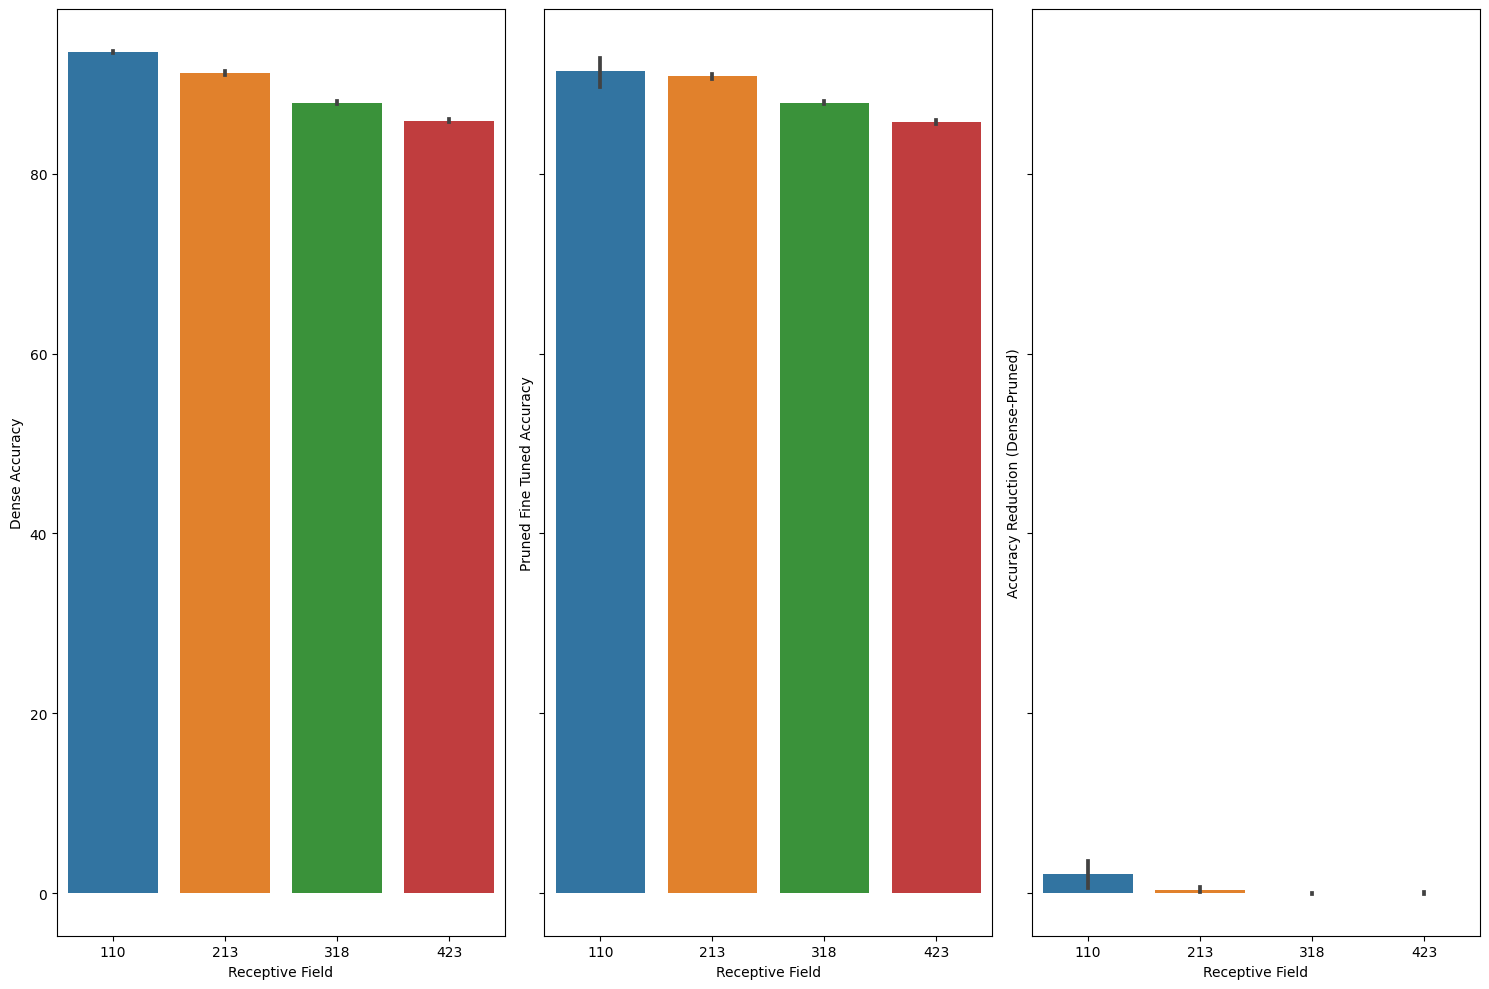
\includegraphics[width=1.1\columnwidth]{images/Supplementary_material/cifar10_vgg19_pruning_finetuned_results_0.9.png}
    \caption{VGG}
    \label{subfig:vgg19CIfar10FInetuned}
     \end{subfigure}
      \hfill
     \begin{subfigure}[b]{\columnwidth}
    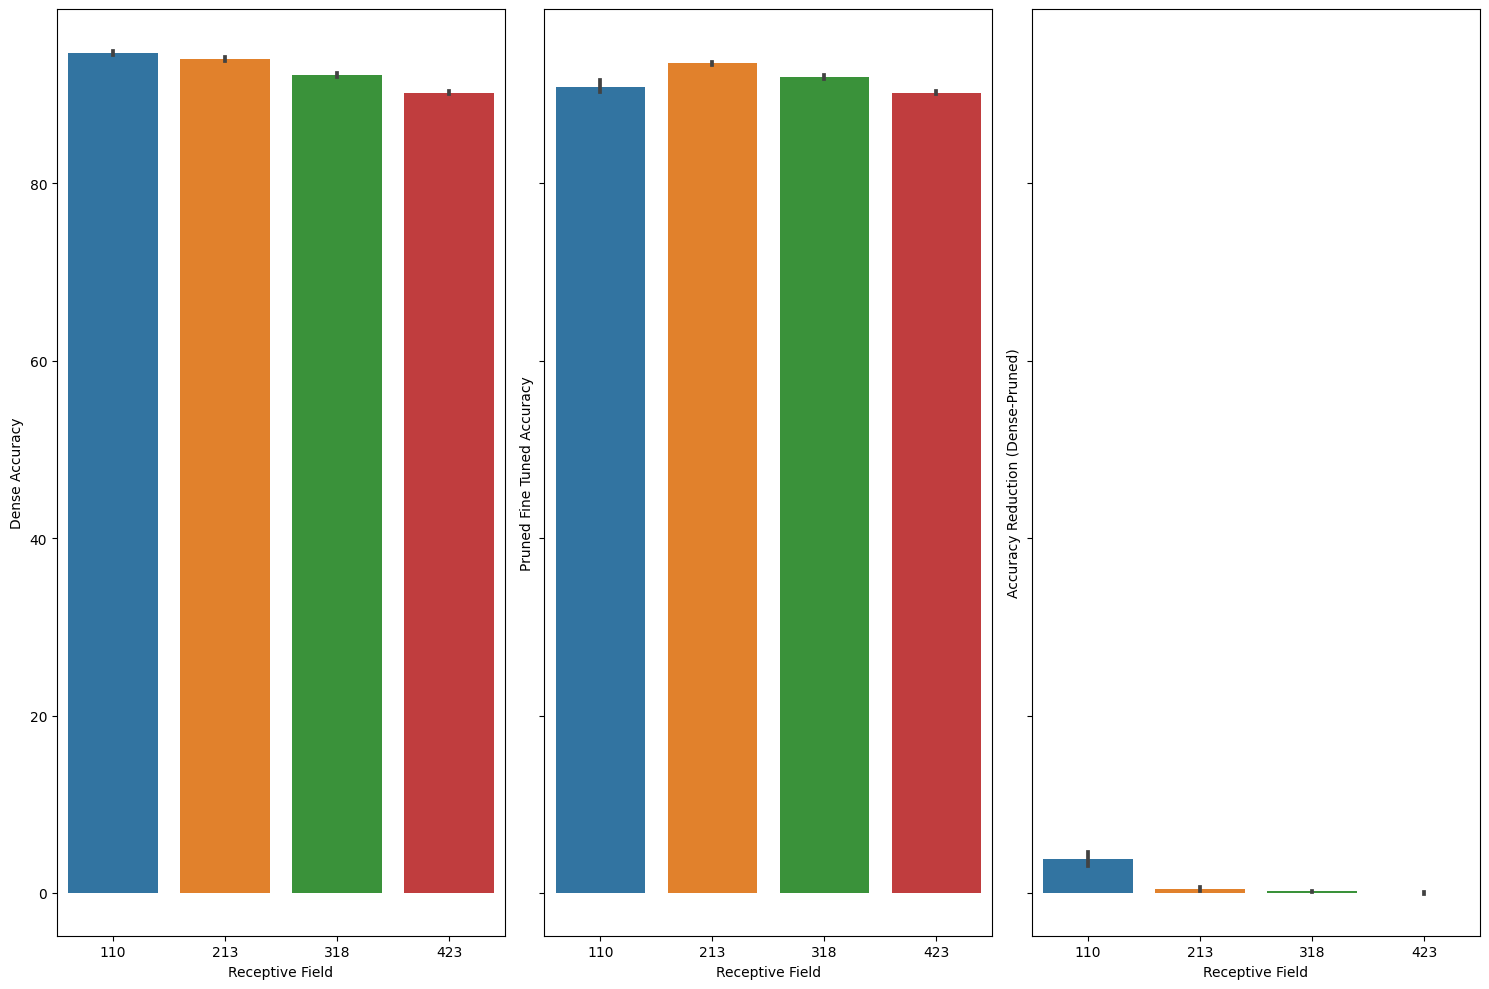
\includegraphics[width=1.1\columnwidth]{images/Supplementary_material/cifar10_resnet50_pruning_finetuned_results_0.9.png}
    \caption{ResNet-50}
    \label{subfig:resenet50CIfar10FInetuned}
     \end{subfigure}
     \caption{ CIFAR10 Fine-tuned results}
    \label{fig:finetuned_CIFAR10}
  \end{figure}

\begin{figure*}[!htb]
 \centering
     \begin{subfigure}[b]{\columnwidth}
    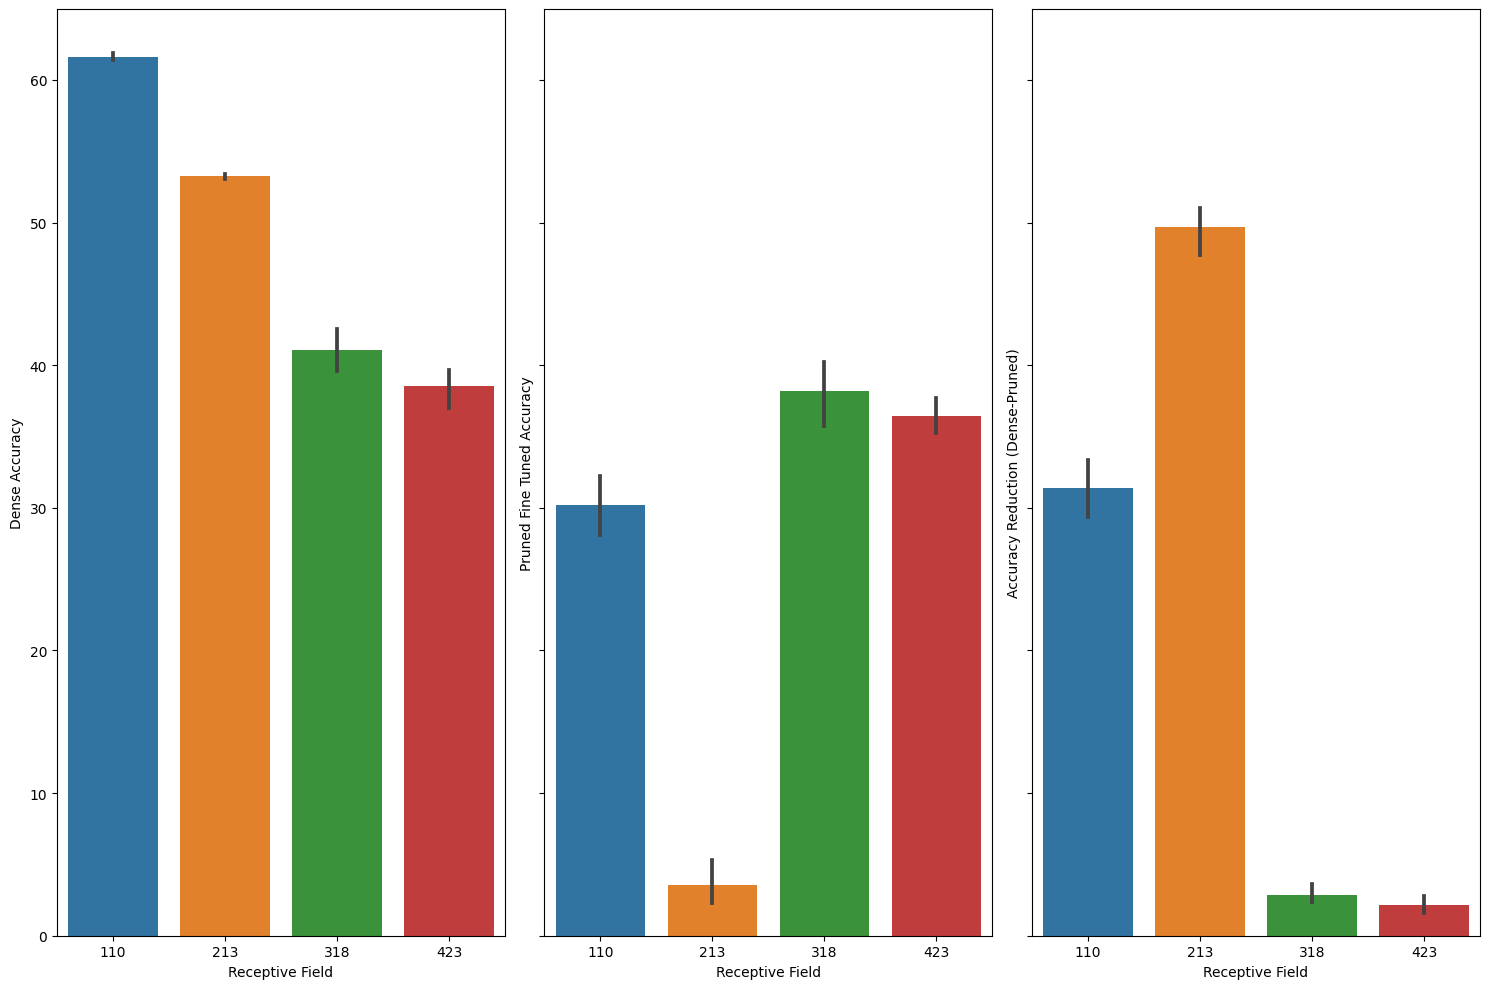
\includegraphics[width=1.1\columnwidth]{images/Supplementary_material/tiny_imagenet_vgg19_pruning_finetuned_results_0.9.png}
    \caption{VGG}
    \label{subfig:vgg19_tiny_imagenet_FInetuned}
     \end{subfigure}
      \hfill
     \begin{subfigure}[b]{\columnwidth}
    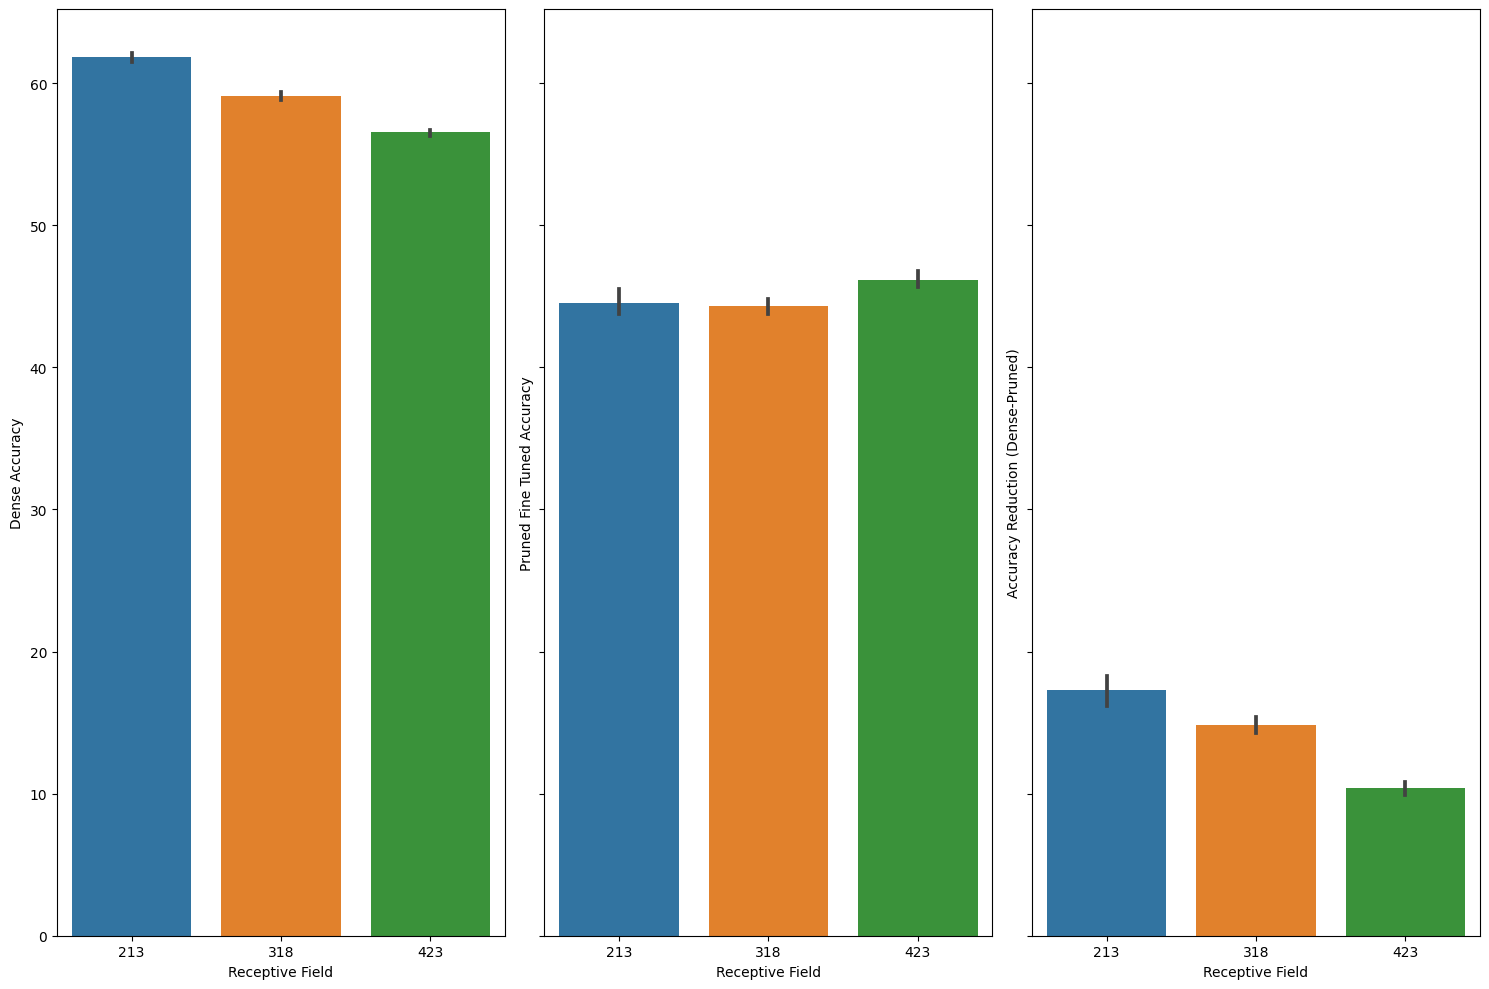
\includegraphics[width=1.1\columnwidth]{images/Supplementary_material/tiny_imagenet_resnet50_pruning_finetuned_results_0.9.png}
    \caption{ResNet-50}
    \label{subfig:resenet50tiny_imagenetFinetuned}
     \end{subfigure}
     \caption{Tiny ImageNet Fine-tuned results}
    \label{fig:finetuned_tiny_imagenet}
\end{figure*}





  \end{document}
